%% 
%% Copyright 2007-2025 Elsevier Ltd
%% 
%% This file is part of the 'Elsarticle Bundle'.
%% ---------------------------------------------
%% 
%% It may be distributed under the conditions of the LaTeX Project Public
%% License, either version 1.3 of this license or (at your option) any
%% later version.  The latest version of this license is in
%%    http://www.latex-project.org/lppl.txt
%% and version 1.3 or later is part of all distributions of LaTeX
%% version 1999/12/01 or later.
%% 
%% The list of all files belonging to the 'Elsarticle Bundle' is
%% given in the file `manifest.txt'.
%% 
%% Template article for Elsevier's document class `elsarticle'
%% with harvard style bibliographic references

\documentclass[review,12pt,authoryear]{elsarticle}

%% Use the option review to obtain double line spacing
%% \documentclass[authoryear,preprint,review,12pt]{elsarticle}

%% Use the options 1p,twocolumn; 3p; 3p,twocolumn; 5p; or 5p,twocolumn
%% for a journal layout:
%% \documentclass[final,1p,times,authoryear]{elsarticle}
%% \documentclass[final,1p,times,twocolumn,authoryear]{elsarticle}
%% \documentclass[final,3p,times,authoryear]{elsarticle}
%% \documentclass[final,3p,times,twocolumn,authoryear]{elsarticle}
%% \documentclass[final,5p,times,authoryear]{elsarticle}
%% \documentclass[final,5p,times,twocolumn,authoryear]{elsarticle}

%% For including figures, graphicx.sty has been loaded in
%% elsarticle.cls. If you prefer to use the old commands
%% please give \usepackage{epsfig}

%% The amssymb package provides various useful mathematical symbols
\usepackage{amssymb}
%% The amsmath package provides various useful equation environments.
\usepackage{amsmath}
%% The amsthm package provides extended theorem environments
%% \usepackage{amsthm}
%% The lineno packages adds line numbers. Start line numbering with
%% \begin{linenumbers}, end it with \end{linenumbers}. Or switch it on
%% for the whole article with \linenumbers.
\usepackage{lineno}

\usepackage{float}

\usepackage{booktabs}

\usepackage{rotating}

%% Allow larger floats to share a page with text (defaults are 0.7/0.3/0.2/0.5)
\renewcommand{\topfraction}{0.85}
\renewcommand{\bottomfraction}{0.70}
\renewcommand{\textfraction}{0.10}
\renewcommand{\floatpagefraction}{0.75}

\graphicspath{{../model_results/}}

\journal{Journal of Hydrology: Regional Studies}

%% --- Document start ---
\begin{document}
%% Add \usepackage{lineno} before \begin{document} and uncomment 
%% following line to enable line numbers
\linenumbers

%% --- Front Matter ---
\begin{frontmatter}

%% Title, authors and addresses

%% use the tnoteref command within \title for footnotes;
%% use the tnotetext command for theassociated footnote;
%% use the fnref command within \author or \affiliation for footnotes;
%% use the fntext command for theassociated footnote;
%% use the corref command within \author for corresponding author footnotes;
%% use the cortext command for theassociated footnote;
%% use the ead command for the email address,
%% and the form \ead[url] for the home page:
%% \title{Title\tnoteref{label1}}
%% \tnotetext[label1]{}
%% \author{Name\corref{cor1}\fnref{label2}}
%% \ead{email address}
%% \ead[url]{home page}
%% \fntext[label2]{}
%% \cortext[cor1]{}
%% \affiliation{organization={},
%%            addressline={}, 
%%            city={},
%%            postcode={}, 
%%            state={},
%%            country={}}
%% \fntext[label3]{}

\title{Can SEAS5 seasonal forecasts drive daily streamflow prediction? Machine learning experiments in Central Asian catchments} %% Article title

%% Authors
\author[1]{Diegopablo Pineda Schwarz\corref{cor1}}
\ead{diegopab@pik-potsdam.de}
\author[1]{Iulii Didovets}
\author[1]{Bijan Fallah}
\author[2]{Tursyn Tillakarim}

\cortext[cor1]{Corresponding author}

%% Author affiliation
\affiliation[1]{organization={Potsdam Institute for Climate Impact Research},%Department and Organization
            addressline={Telegraphenberg A31}, 
            city={Potsdam},
            postcode={14473}, 
            state={Brandenburg},
            country={Germany}}

\affiliation[2]{organization={Research Center, Republican State Enterprise ``Kazhydromet''},%Department and Organization
            addressline={Mangilik El Avenue 11/1},
            city={Astana},
            postcode={010000},
            country={Kazakhstan}}


\begin{abstract}

\textbf{Study Region:} Seven Central Asian catchments in two regimes: nival--glacial mountain catchments in Tajikistan and Kazakhstan (Zeravshan, Ulken Boken, Kurshim) and nival-dominated rainfed steppe catchments in Kazakhstan (Esil, Ayat, Kalkutan, Zhabay), plus two European Alpine catchments (Kirchbichl--Bichlwang, Diepoldsau--Rietbr\"ucke) for out-of-region validation.

\textbf{Study Focus:} We test whether ECMWF's openly available SEAS5 seasonal forecast carries usable information for daily discharge prediction at lead times up to 214 days. Ridge regression, Random Forest, XGBoost and an LSTM network were trained to predict the log-transformed discharge anomaly relative to the day-of-year climatology and evaluated by leave-one-year-out cross-validation against climatology, persistence and damped-persistence baselines. Models were compared untuned, after nested-CV tuning, and under corrupted forcing.

\textbf{New Hydrological Insights for the Region:} Every forecast, climatology included, reached high median Nash--Sutcliffe efficiencies in the nival--glacial mountain catchments (0.85--0.91 at Zeravshan), as volumetric metrics reward reproduction of the seasonal cycle. On anomaly scores, however, no learned model significantly outperformed damped persistence there, and tuning improved only the tree ensembles, without closing the gap. In the steppe catchments anomaly skill was carried by persistence: the models beat damped persistence only at long leads, after it had lost its skill, but their volumetric accuracy collapsed. Donor-year forcing changed every median score by at most 0.012: the models rely on the antecedent discharge anomaly, not the forecast weather. Damped persistence therefore remains the benchmark to beat, and anomaly scores assessed against a persistence reference are the honest measure of skill where climatology dominates.

\end{abstract}

\begin{graphicalabstract}
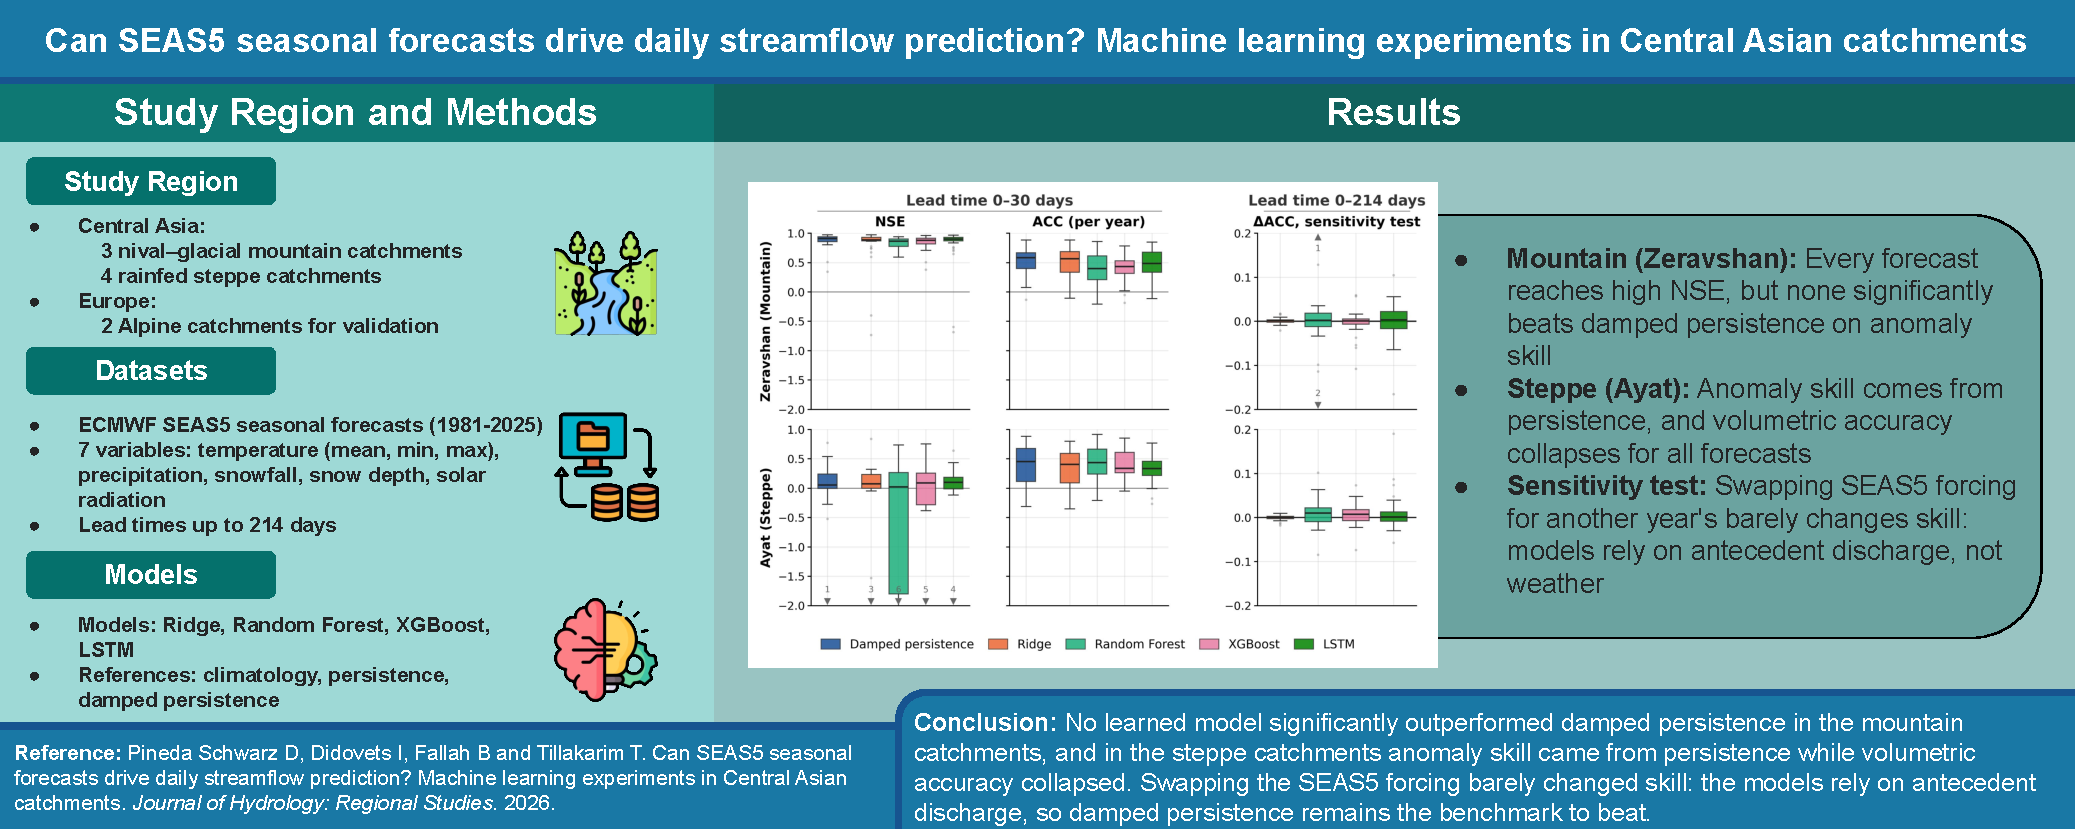
\includegraphics[width=\linewidth]{00_plots/Graphical_Abstract.pdf}
\end{graphicalabstract}

\begin{highlights}
\item No learned model significantly beat damped persistence in nival–glacial catchments.
\item In steppe catchments, anomaly skill came from persistence, not the learned models.
\item Donor-year forcing left skill intact: models use antecedent discharge, not weather.
\item Where the seasonal cycle dominates, climatology alone reaches high NSE and KGE.
\end{highlights}

\begin{keyword}
%% keywords here, in the form: keyword \sep keyword
Seasonal streamflow forecasting \sep Central Asia \sep SEAS5 \sep Machine learning \sep Forecast verification \sep Snow-dominated catchments

%% PACS codes here, in the form: \PACS code \sep code
%% MSC codes here, in the form: \MSC code \sep code
%% or \MSC[2008] code \sep code (2000 is the default)

\end{keyword}

\end{frontmatter}

\section{Introduction}
\label{sec:intro}

Water is a critical resource in Central Asia, where agriculture accounts for up to 82\% of freshwater withdrawal, with the remainder split between industrial (10\%) and municipal (8\%) use \citep{hernandez2025}. This heavy reliance on agriculture makes the region highly dependent on effective water management. The extensive irrigation network built during the Soviet era once connected all Central Asian countries into a single, coordinated system; however, following the Soviet collapse, the network remained in use even as the resources and institutional capacity required for its maintenance disappeared. Since independence, each country has prioritized its own water and food security, complicating efforts to manage the shared system fairly and consistently \citep{ohara2000, bamgboye2025}. This governance challenge has been compounded in recent decades by rapid urbanization and development, which have intensified water scarcity across the region. Climate change poses a further threat, driving accelerated glacier loss and increasingly unstable runoff patterns that, together with the lack of unified governance, risk exacerbating existing water scarcity issues \citep{guo2024, zhang2026}. Most agricultural irrigation water originates as snow and glacier melt in the high mountain ranges of the Tien Shan and Pamir, from which it flows into the lowland river systems that sustain regional agriculture. Because river discharge is governed directly by snow accumulation and glacier melt dynamics, glacier monitoring efforts have been established to help anticipate changes in discharge patterns \citep{zhang2026, barandun2021}. Direct measurement tools, such as the water gauge stations at catchment sites, are essential for local water management, providing continuous records of discharge that inform day-to-day operational decisions. However, extending this monitoring capability with reliable seasonal forecasts of river discharge at the catchment scale would allow local communities to anticipate wet or dry events before they occur, providing an invaluable asset for water resource management during abnormal climatic conditions.

There are two principal approaches to seasonal discharge forecasting: physically-based hydrological models and machine learning models. Physically-based models encode mechanistic understanding, simulating the physical laws and processes that govern snow accumulation, glacier melt, and runoff generation within a catchment. This mechanistic grounding provides strong interpretability and allows for physically consistent extrapolation beyond observed conditions, but it comes at a cost: these models typically require high-resolution spatial and temporal input data, along with sufficiently long and reliable observational records for calibration and validation, both of which are often scarce in remote or poorly instrumented regions such as Central Asia. Data-driven machine learning models, on the other hand, trade interpretability for flexibility and lower input requirements. Rather than explicitly modeling physical processes, these models learn statistical relationships directly from historical data, functioning largely as a "black box" with limited insight into the underlying mechanisms. This flexibility, however, makes machine learning approaches particularly well suited to data-scarce settings, where the sparse observational networks and limited historical records would otherwise constrain physically-based modeling \citep{jin2024, liang2023, sayed2023, mohammadi2021}.

Previous studies in Central Asia have applied statistical and machine learning methods to forecast river discharge, though rarely with lead times spanning a full season (~6 months) at daily resolution. Simple linear-regression-based forecasts of seasonal (April–September) mean discharge have been developed for multiple catchments across the region and form the basis of current operational practice at national hydromet agencies \citep{apel2018}. More recent work has introduced machine learning techniques, such as random forest, Gaussian process, and support vector regression, to forecast the same April–September seasonal mean discharge using snow water equivalent and climate oscillation indices as predictors \citep{umirbekov2025}. Other studies have applied machine learning at shorter, sub-seasonal horizons, such as daily, 5-day, and 10-day periods, using a variety of techniques including LSTM, XGBoost, and SVR, among others \citep{ji2021, abdoulhalik2024, hunziker2026}. A gap nonetheless remains in the application of machine learning to daily-resolution discharge forecasting at seasonal lead times (~6 months) in Central Asia, driven primarily by the limited availability of seasonal-length climate forcing data required to drive such models beyond the short lead times supported by simpler persistence- or antecedent-condition-based predictors. A recent study in North America addressed an analogous gap by using ECMWF's SEAS5 product to drive machine learning models at seasonal lead times \citep{swiftlapointe2025}. SEAS5 is particularly well suited to this purpose, and to the needs of hydromet agencies more broadly, as it is open-source, freely accessible, and sustainably maintained, while offering daily-resolution climate forcing data at a global scale with lead times of up to 215 days \citep{copernicus2018}. Building on the approach of \citet{swiftlapointe2025}, the present study addresses the corresponding gap in Central Asia through the use of ECMWF's SEAS5 seasonal forecast product, applying it to drive machine learning models for full-season discharge forecasting in the region.

In this study, we evaluate whether SEAS5 seasonal forecasts carry usable information for daily-resolution discharge prediction at seasonal lead times, addressing the gap identified above. We train four models, Ridge regression, Random Forest, XGBoost, and an LSTM, to predict discharge anomalies relative to the local seasonal cycle, rather than raw discharge, at lead times of up to 214 days. Models are applied across catchments spanning three hydrological regimes: nival-glacial-dominated mountain catchments and nival-dominated steppe catchments in Central Asia, together with nival-glacial-dominated European catchments included for out-of-region comparison. Model development proceeds in three stages: an initial comparison of all models and catchments at default settings, a hyperparameter tuning stage to assess the extent to which model performance can be improved on a per-catchment basis, and a sensitivity test that corrupts the meteorological forcing at inference time to determine whether model skill genuinely derives from the forecast weather or merely reflects the seasonal cycle. Together, these stages offer insight into whether, and under what conditions, machine learning models trained on SEAS5 forecasts can meaningfully improve on simpler forecasting strategies in strongly climatology-dominated catchments.

\subsection{Study Area}

The study comprises a total of seven river catchments, broadly classified into two hydrological regimes: Central Asian nival-glacial-dominated mountain catchments (Zeravshan, Ulken Boken, Kurshim), and Central Asian nival-dominated, rainfed steppe catchments (Esil, Ayat, Kalkutan, Zhabay). An additional two catchments were included as an out-of-region validation subset: European nival-glacial-dominated mountain catchments (Kirchbichl-Bichlwang, Diepoldsau-Rietbruecke). Figure~\ref{fig:catchments} displays the location of each catchment. For brevity, the results presented in the main text are restricted to one representative catchment per regime: Zeravshan, Ayat, and Kirchbichl-Bichlwang, respectively. Table~\ref{tab:catchments} summarizes the general characteristics of these rivers.

\begin{table}[h]
    \centering
    \small
    \setlength{\tabcolsep}{3.5pt}
    \begin{tabular}{llccc}
        \toprule
        \textbf{River} & \textbf{Station} & \textbf{Area} & \textbf{Mean discharge} & \textbf{SEAS5 cells} \\
        \midrule
        \multicolumn{5}{l}{\textit{Central Asia (primary study region)}} \\
        Zeravshan   & Dupuli          & 10{,}200 & 158.1 & 3$\times$4 (12) \\
        Ulken Boken & Zhumba          & 758      & 8.2   & 2$\times$2 (4) \\
        Kurshim     & Voznesenskoje   & 5{,}840  & 75.6  & 2$\times$4 (8) \\
        Esil        & Turgenevka      & 3{,}240  & 5.3   & 1$\times$2 (2) \\
        Ayat        & Varvarinka      & 10{,}300 & 6.9   & 2$\times$4 (8) \\
        Kalkutan    & Qalaotan        & 16{,}500 & 6.0   & 2$\times$3 (6) \\
        Zhabay      & Atbasar         & 8{,}530  & 14.1  & 2$\times$3 (6) \\
        \addlinespace
        \multicolumn{5}{l}{\textit{Europe}} \\
        Inn         & Kirchbichl-Bichlwang     & 9{,}310 & 292.1 & 2$\times$4 (8) \\
        Rhine       & Diepoldsau-Rietbr\"ucke  & 6{,}119 & 230.2 & 2$\times$3 (6) \\
        \bottomrule
    \end{tabular}
    \caption{Physical and hydrological characteristics of the studied river catchments \citetext{\citealp{grdc2026}; Kazhydromet, unpublished data, 2025; Tajik Hydromet, unpublished data, 2025}. SEAS5 cells: the $1^\circ\times1^\circ$ grid cells averaged into each catchment's forcing.}
    \label{tab:catchments}
\end{table}


The nival-glacial-dominated mountain catchments, namely Zeravshan, Ulken Boken, Kurshim, Kirchbichl-Bichlwang, and Diepoldsau-Rietbruecke, are characterized by highly regular seasonal cycles, driven by the consistent yearly pattern of snow accumulation in winter and snow and glacier melt in summer at the high elevations where these rivers originate. Because melting progresses through the mountains at different times as warming reaches successively higher elevations, this regulating effect produces comparatively low variability in annual runoff \citep{siegfried2024}.

The nival-dominated steppe catchments, namely Esil, Ayat, Kalkutan, and Zhabay, behave differently. These catchments are fed primarily by snowmelt and rainfall from low mountains, and discharge large volumes of water over short periods, concentrated around the peak of snowmelt. Rivers in this regime typically dry up over the summer, once the accumulated snowpack has fully melted and groundwater supplies decline \citep{siegfried2024}.

\begin{figure}[H]
    \centering
    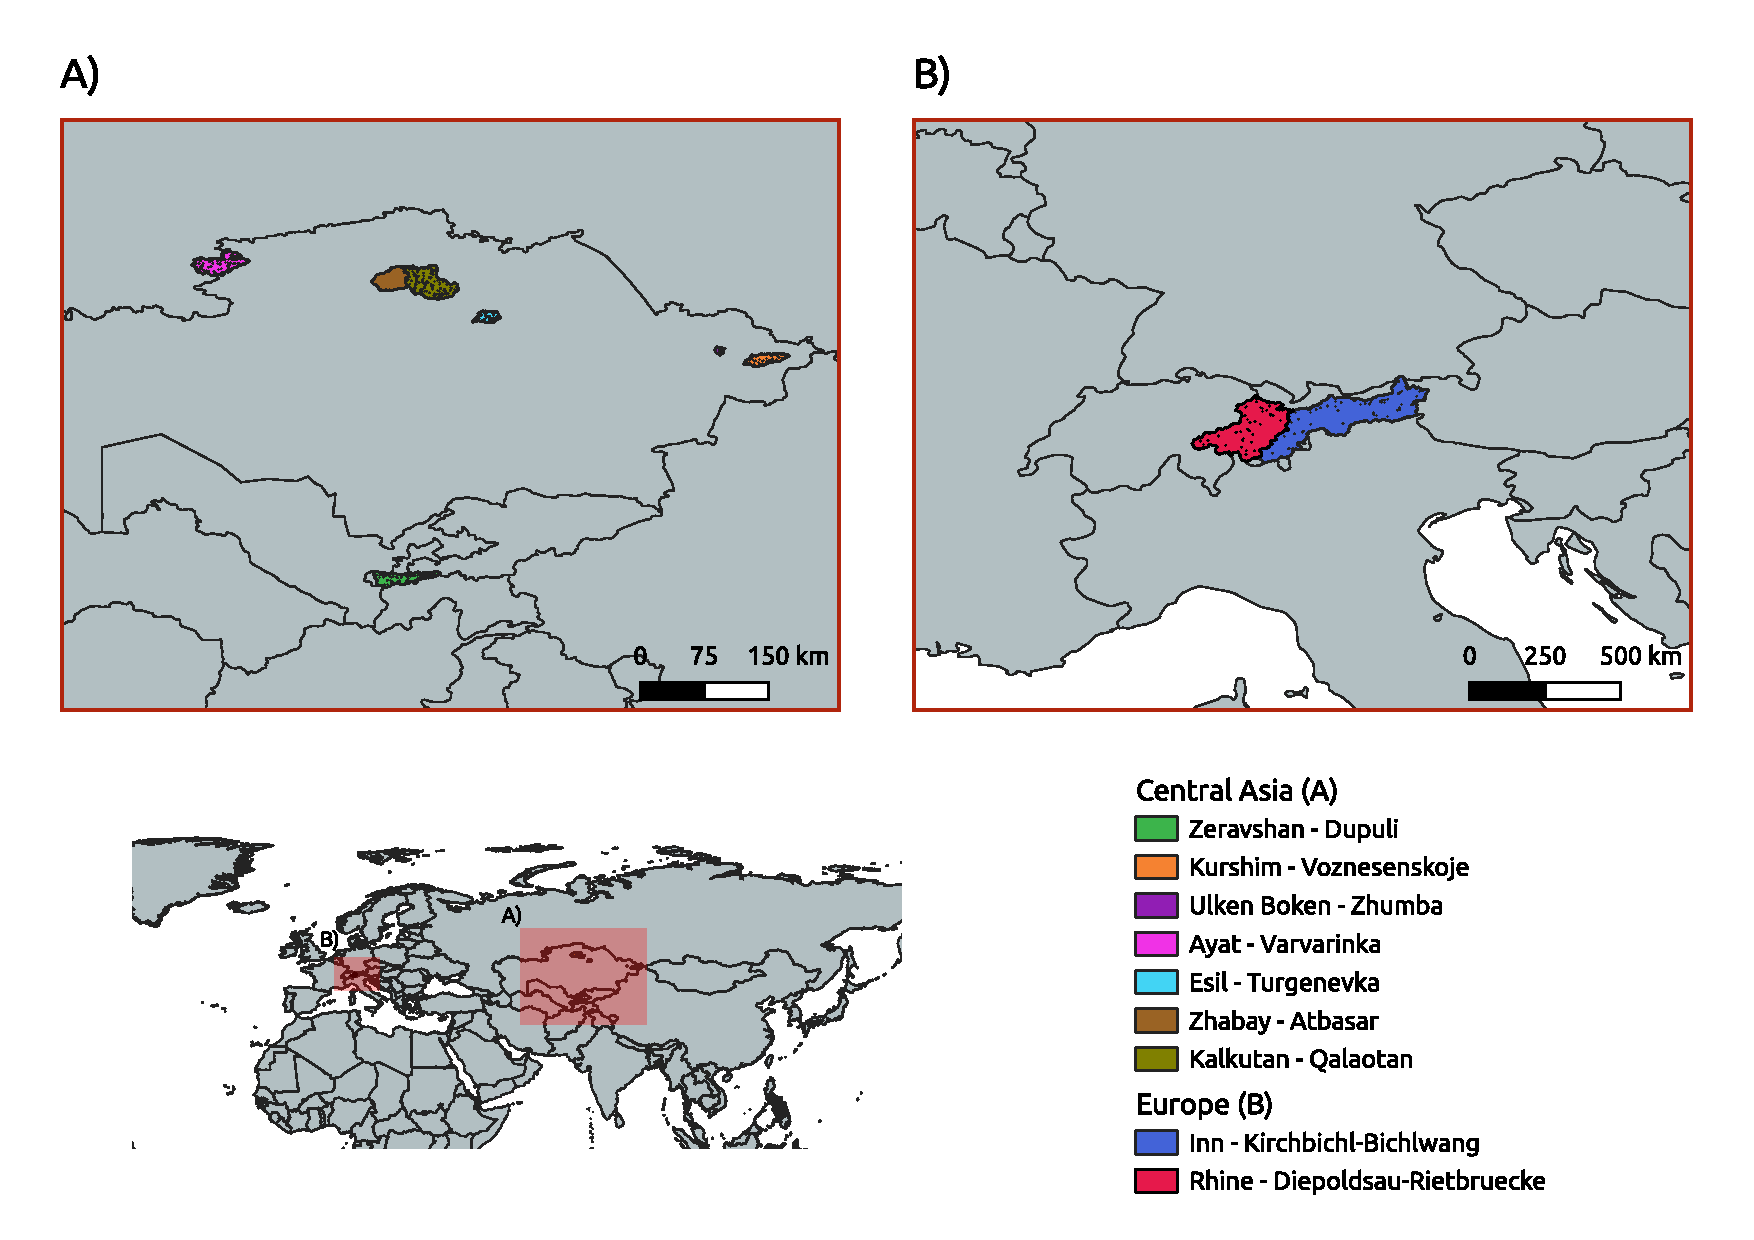
\includegraphics[width=\textwidth]{00_plots/fig01.pdf}
    \caption{Boundaries of the nine study catchments, labelled by river and gauging station: (A) Central Asian catchments in Kazakhstan and Tajikistan; (B) Additional alpine catchments in Europe.}
    \label{fig:catchments}
\end{figure}



\section{Methods}
\label{sec:methods}

The study evaluates whether seasonal meteorological forecasts carry usable information for predicting river discharge at seasonal lead times. Daily discharge observations are paired with ensemble forcing from the ECMWF SEAS5 seasonal forecasting system, and four statistical and machine-learning models are trained to predict the discharge anomaly relative to the local seasonal cycle at lead times of up to 214 days. Skill is measured against climatological and persistence baselines under leave-one-hydrological-year-out cross-validation. Model development then proceeds in three stages. The first compares all four models, together with the reference baselines, at their default settings across every catchment, establishing an untuned reference. The second tunes the model hyperparameters within a nested cross-validation, quantifying how much is gained by adapting a model to an individual catchment rather than leaving it at its defaults. The third corrupts the meteorological input at inference time and measures the resulting loss of skill, testing whether the forecasts genuinely draw on the weather or merely reproduce the seasonal cycle. Figure~\ref{fig:schematic} summarises the workflow.

\begin{figure}[!htbp]
    \centering
    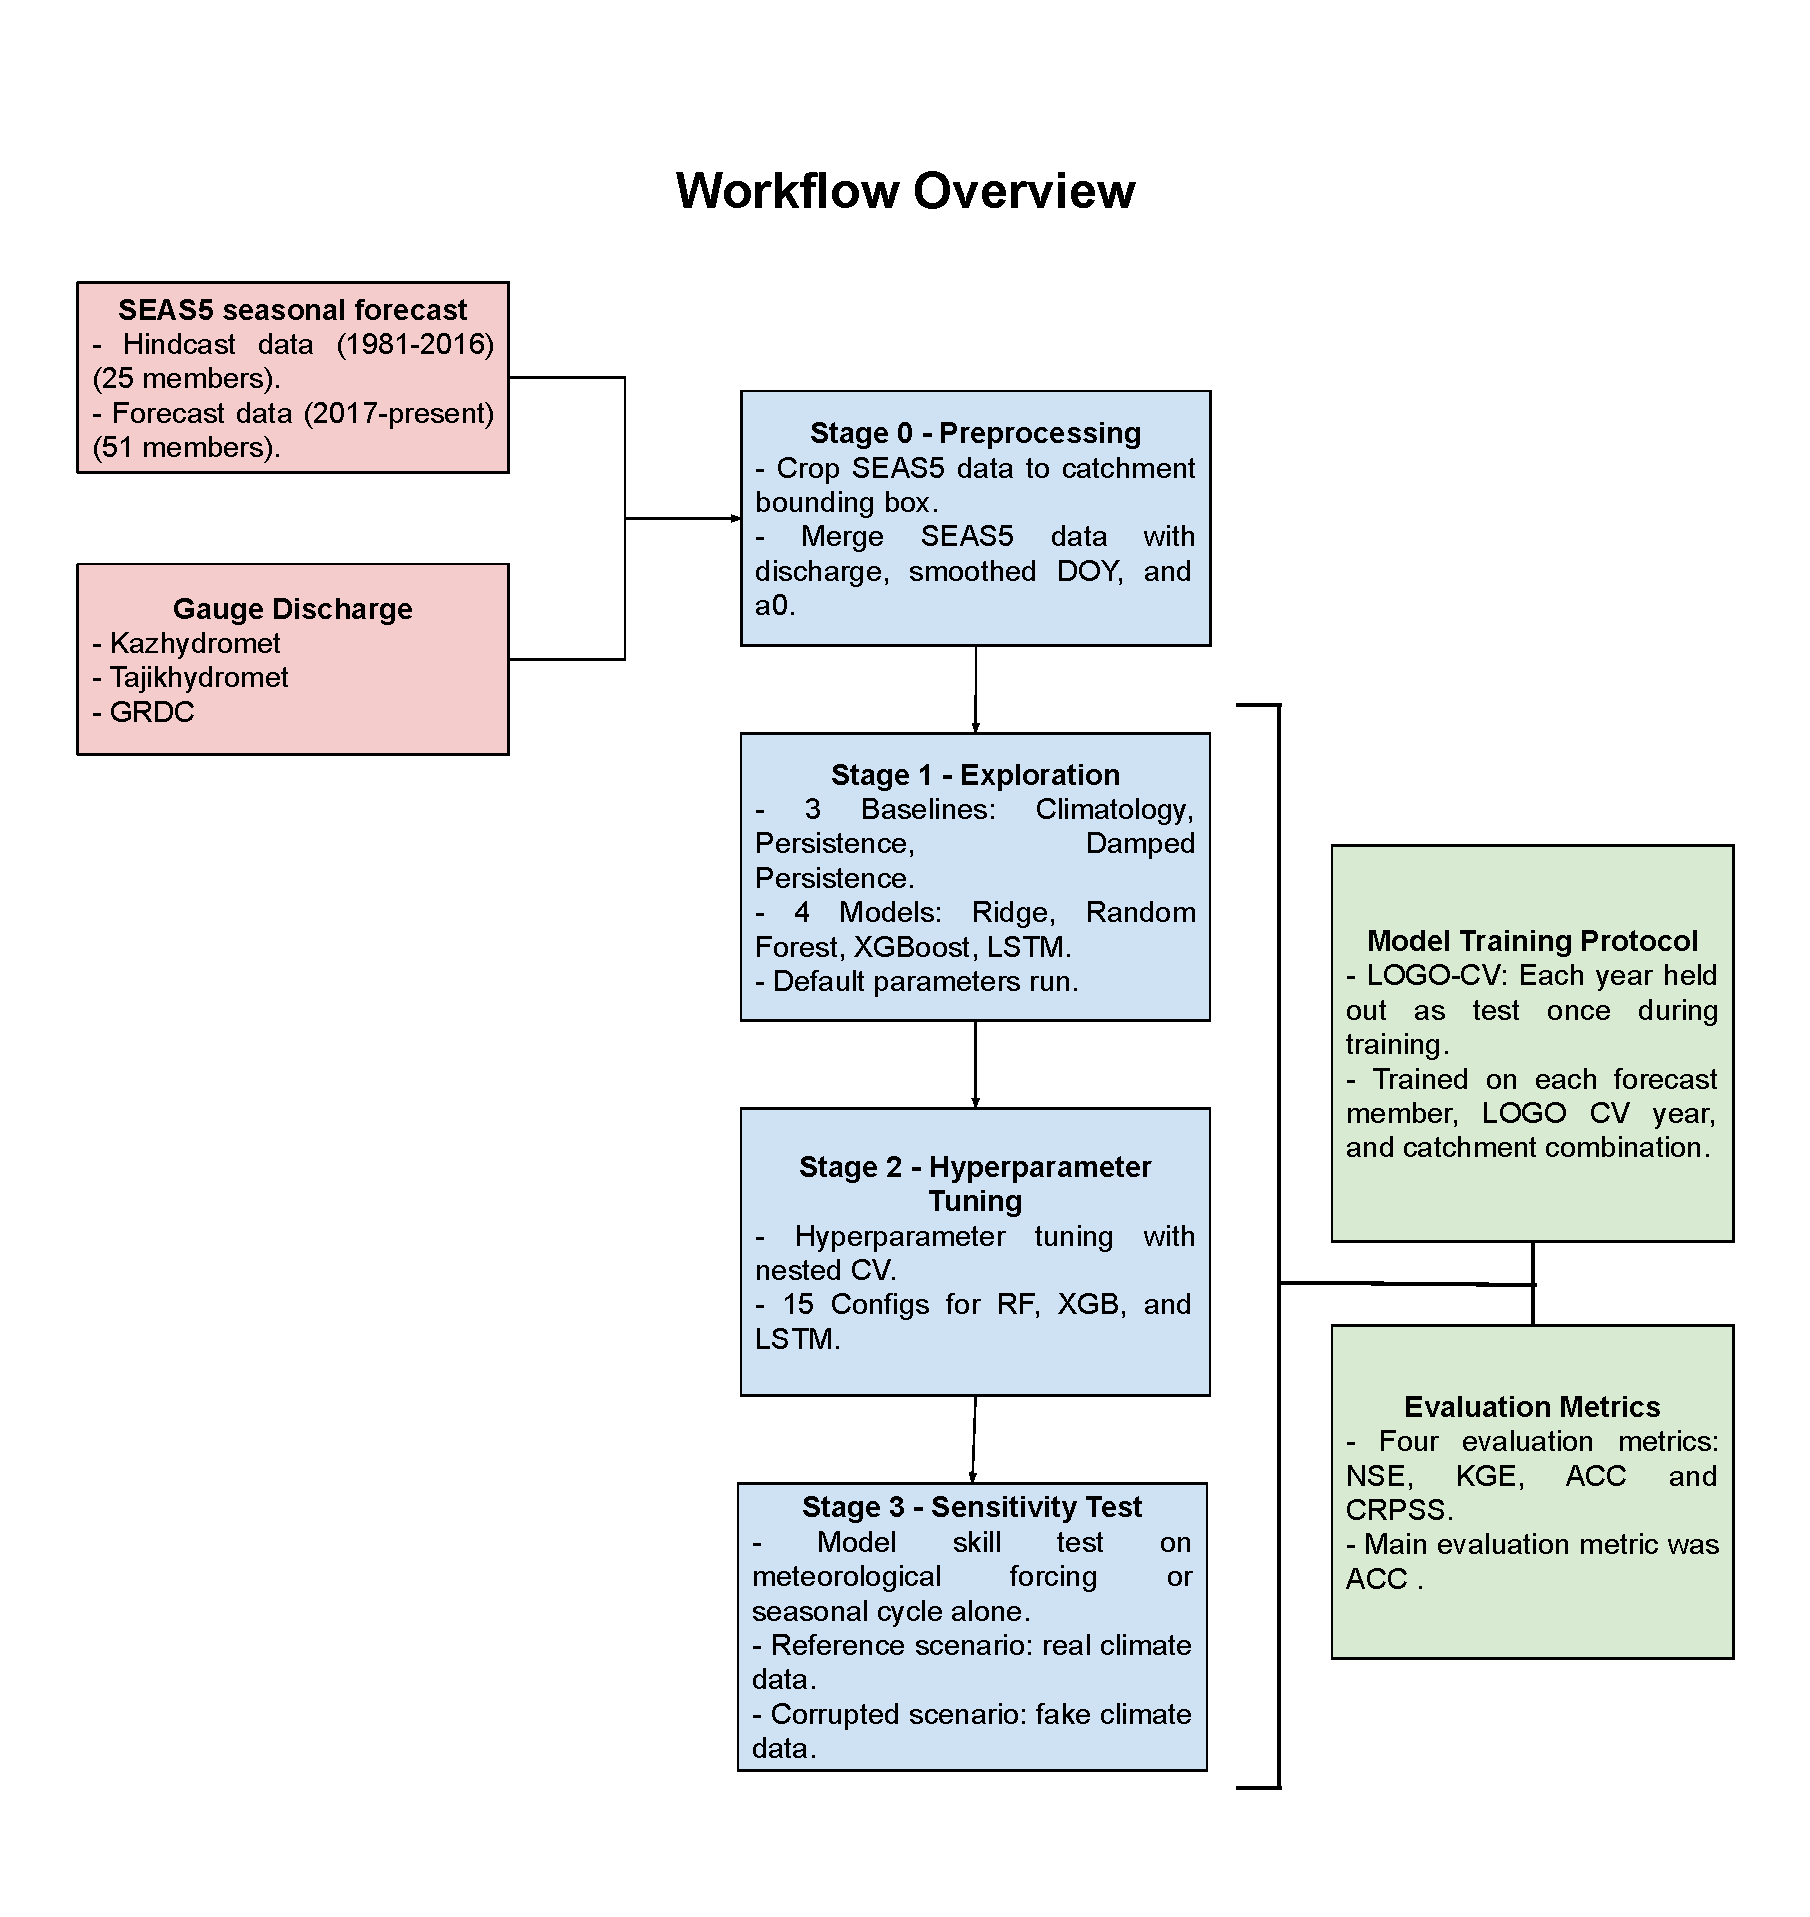
\includegraphics[height=0.6\textheight,keepaspectratio]{00_plots/fig02.pdf}
    \caption{Schematic of the modelling workflow, from SEAS5 and discharge preprocessing to the three experimental stages.}
    \label{fig:schematic}
\end{figure}

Every stage described below was run for all nine catchments described in the study area. The results presented in the main text are restricted to one representative catchment per regime (Zeravshan, Ayat, and Kirchbichl-Bichlwang); results for all nine catchments are given in \ref{app:stage1}, \ref{app:stage2} and \ref{app:stage3}.

\subsection{Data Sourcing and Preprocessing}

Daily discharge observations were obtained from Kazhydromet (Kazhydromet, unpublished data, 2025), Tajik Hydromet (Tajik Hydromet, unpublished data, 2025), and the Global Runoff Data Centre \citep{grdc2026}. Per-catchment details are listed in Table~\ref{tab:catchments}. The hydrological year was defined as starting 1 October, so each year spans one full snow accumulation and melt cycle. Years with missing data or due to low quality were excluded from training and evaluation.

Atmospheric forcing was taken from the ECMWF Seasonal Forecast System 5 (SEAS5), accessed through the Copernicus Climate Data Store \citep{copernicus2018}. SEAS5 provides ensemble forecasts on a 1$^{\circ}$~$\times$~1$^{\circ}$ global grid, initialised on the first day of each month. Data between 1981 and 2016 are hindcasts, containing 25 ensemble members, while data between 2017 and 2025 are operational forecasts, containing 51 ensemble members; the full ensemble was retained in both cases. Data were downloaded over 1981--2025 for both a Central Asian domain (34$^{\circ}$N--58$^{\circ}$N, 46$^{\circ}$E--88$^{\circ}$E) and a European domain (35$^{\circ}$N--59$^{\circ}$N, 11$^{\circ}$W--26$^{\circ}$E), retaining the full 215-day lead time of every initialisation. Seven variables were extracted: mean, maximum and minimum 2~m air temperature; downwelling surface solar radiation; total precipitation; snow depth; and snowfall. 

For each catchment, SEAS5 fields were cropped to a bounding box enclosing the basin and reduced to one time series per variable and ensemble member by a cosine-latitude-weighted spatial mean. Sub-daily forecast steps were averaged to daily resolution. Four further predictors were derived. The first two encode the seasonal cycle: the day of year (DOY) was mapped onto $\sin(2\pi\,\mathrm{DOY}/365.25)$ and $\cos(2\pi\,\mathrm{DOY}/365.25)$, which preserve continuity across the year boundary. The third, $a_{0}$, is the antecedent discharge anomaly: the $\log(1+Q)$-transformed discharge observed on day~0 of the forecast, minus the smoothed day-of-year discharge climatology at that date. It expresses how far the catchment departed from its seasonally expected state at initialisation, instead of providing the models with the raw discharge values. The fourth is the lead day, from 0 to 214. The three tabular models therefore receive eleven predictors; the LSTM receives ten, omitting the lead day, which the position of a timestep within the sequence already encodes.

\subsection{Cross-Validation and Evaluation}

Model skill was assessed by leave-one-hydrological-year-out cross-validation (LOGO-CV), applied identically to the four models. Each record was assigned to the hydrol
ogical year of its verification date, and every hydrological year in the catchment's record was withheld in turn as the test set while the model was fitted on all remaining years. A catchment with $N$ hydrological years therefore yields $N$ folds. Folds are constructed once under a fixed random seed and shared by every model, so that fold-wise scores can be compared pairwise.

All quantities estimated from data are estimated within the fold: the standardisation statistics of the predictors, the regularisation strength of the Ridge model, and all fitted model parameters were determined on the training years alone and applied unchanged to the held-out year. The single exception is the day-of-year discharge climatology that defines the anomaly target and $a_{0}$. It is computed once per catchment as the mean of $\log(1+Q)$ on each day of year over the observed years from 1981 onward, the period covered by SEAS5, smoothed with a centred 31-day moving window applied circularly across the year boundary. Refitting it per fold would give each fold a slightly different anomaly definition and a different reference for the anomaly correlation.

Model performance was assessed with four metrics, each computed once per fold (test hydrological year) and then aggregated across folds. Let $Q_t$ and $\hat{Q}_t$ denote observed and predicted (ensemble-mean) discharge on day $t$ of the evaluation window, with $T$ days in total. The Nash--Sutcliffe efficiency \citep[NSE;][]{nash1970} and the Kling--Gupta efficiency \citep[KGE;][]{gupta2009} were evaluated in discharge space:
\begin{equation}
\mathrm{NSE} = 1 - \frac{\sum_t (\hat{Q}_t - Q_t)^2}{\sum_t (Q_t - \bar{Q})^2}, \qquad
\mathrm{KGE} = 1 - \sqrt{(r-1)^2 + (\alpha-1)^2 + (\beta-1)^2},
\end{equation}
where $r$ is the Pearson correlation between $\hat{Q}$ and $Q$, $\alpha = \sigma_{\hat{Q}}/\sigma_Q$ and $\beta = \mu_{\hat{Q}}/\mu_Q$.

The anomaly correlation coefficient \citep[ACC;][]{jolliffe2012} is taken as the main performance metric. It is the centred Pearson correlation between predicted and observed anomalies, computed in the same space as the models' target, with anomalies defined relative to the smoothed day-of-year climatology $c_t$ of $\log(1+Q)$:
\begin{equation}
\mathrm{ACC} = \frac{\sum_t (a_t - \bar{a})(\hat{a}_t - \bar{\hat{a}})}{\sqrt{\sum_t (a_t - \bar{a})^2 \sum_t (\hat{a}_t - \bar{\hat{a}})^2}}, \qquad
a_t = \log(1+Q_t) - c_t, \quad \hat{a}_t = \log(1+\hat{Q}_t) - c_t.
\end{equation}
where $\bar{a}$ and $\bar{\hat{a}}$ are the mean anomalies over the evaluation window, so that ACC measures agreement in the day-to-day variation of the anomalies rather than in their overall level.


The continuous ranked probability score \citep[CRPS;][]{hersbach2000} was computed in discharge space from the $N$ individual ensemble members $\hat{Q}_t^{(i)}$:
\begin{equation}
\mathrm{CRPS} = \frac{1}{T}\sum_t \left[ \frac{1}{N}\sum_{i} \bigl|\hat{Q}_t^{(i)} - Q_t\bigr| - \frac{1}{2N^2}\sum_{i,j} \bigl|\hat{Q}_t^{(i)} - \hat{Q}_t^{(j)}\bigr| \right],
\end{equation}
which reduces to the mean absolute error for a deterministic forecast. The CRPS skill score is $\mathrm{CRPSS} = 1 - \mathrm{CRPS}/\mathrm{CRPS}_{\mathrm{clim}}$, with the day-of-year climatology as reference.

Three deterministic baselines were evaluated under identical folds and metrics, and define the reference the learned models must clear. Climatology predicts a zero anomaly at every lead day, i.e.\ the smoothed seasonal cycle itself; its anomaly is zero by construction, so it has no ACC. Persistence carries the discharge anomaly observed at initialisation, $a_{0}$, forward unchanged across the entire forecast horizon. Damped persistence decays that same anomaly geometrically with lead time, at a rate given by the lag-1 autocorrelation of the catchment's observed anomaly record, estimated once per catchment from contiguous daily pairs over the same period as the climatology, defined using 1981 onward ($\phi$ ranges $0.96$--$0.98$ in the Central Asian catchments and $0.83$--$0.86$ in the Alpine ones).

In addition, a day-of-year reference is shown in every ACC panel as a horizontal line at its median across folds. For each fold it predicts, on every date, the mean of $\log(1+Q)$ on that day of year over the training years, without smoothing, and it is scored with the same ACC, against the same climatology, as every other forecast. Because the 31-day climatology flattens short-lived features of the seasonal cycle, part of the seasonal cycle remains in the anomalies, and a forecast that resolves it more finely earns a positive ACC without any information about the year being forecast. The day-of-year reference measures that level, so it is ACC above this line, rather than above zero, that indicates skill beyond the seasonal cycle.

\subsection{Experiments}

Four models were compared with respect to their skill in predicting river discharge: Ridge regression, Random Forest, XGBoost, and a Long Short-Term Memory (LSTM) network \citep{hochreiter1997}. They were chosen as representatives of distinct machine learning model families: Ridge regression as a basic linear model, Random Forest for bagged decision-tree ensembles, XGBoost for gradient-boosted decision-tree ensembles, and the LSTM for recurrent neural networks. All four share the same prediction task: rather than predicting discharge directly, each model predicts the $\log(1+Q)$ anomaly relative to the smoothed day-of-year climatology of the catchment, which is subsequently back-transformed to discharge and clipped at zero before NSE, KGE and CRPS are computed. This back-transformation carries a known low bias. Adding a predicted anomaly to the climatological mean of $\log(1+Q)$ and inverting the transform recovers a geometric-type rather than an arithmetic mean, so predicted volumes are systematically low, increasingly so as the discharge record becomes more skewed. The bias is documented rather than corrected, since correcting it would mean abandoning the log-anomaly formulation. Predictors were standardised to zero mean and unit variance, using means and standard deviations computed on each fold's training years alone and applied unchanged to the held-out year. Each ensemble member was treated as an independent training sample, and member predictions were averaged at evaluation time.

  \subsubsection{Model Exploration}

The first stage applies the four models, together with the three reference baselines, to every catchment, establishing their untuned performance and exposing how far skill varies from catchment to catchment. The design runs one independent run per catchment and model pair, each executing the complete leave-one-hydrological-year-out cross-validation described above.

At this stage the models are left untuned: Random Forest and XGBoost at their library defaults, and Ridge regression selecting its regularisation strength within each training fold. The LSTM has no library default and is therefore specified explicitly: input features are mapped by a linear layer to a 128-dimensional representation, passed through two stacked LSTM layers of 128 hidden units with a dropout of 0.2 between them, and reduced to a scalar by a head consisting of layer normalisation, dropout, and two fully connected layers with a ReLU activation in between. The hidden state is initialised to zero at every initialisation date. A trajectory crossing 1~October spans two hydrological years; the LSTM always reads it whole from initialisation, and only the timesteps verifying in the years being fitted or evaluated enter the loss or the scores. The remaining timesteps supply only inputs known at initialisation (SEAS5 forcing and $a_{0}$), never a discharge target. Training used the Adam optimiser at an initial learning rate of $3\times10^{-4}$ and a weight decay of $10^{-4}$, in batches of 512 sequences, minimising a Nash--Sutcliffe-form loss computed directly in anomaly space with gradient norms clipped at 1.0. Training ran for at most 50 epochs against a validation split of 15\,\% of the fold's training hydrological years (fixed seed), with the learning rate halved after five epochs without improvement and training stopped after twenty.

Results for this stage are reported as follows. Skill is compared within two 30-day lead-time windows, at the start and end of the forecast (0--30 and 185--214~days), and is shown as the distribution across cross-validation folds rather than a single aggregate, with the day-of-year reference marked in each ACC panel. Because binning by lead time alone confounds the initialisation month, ACC is additionally disaggregated by initialisation month against the seven lead-time bins.

  \subsubsection{Hyperparameter Tuning}

The second stage quantifies how much skill is gained by tuning a model to an individual catchment. Tuning and evaluation are separated by a nested cross-validation, so that no hydrological year both selects a configuration and reports its score. The outer loop is the leave-one-hydrological-year-out scheme described above. Within each outer fold the remaining years are partitioned into five disjoint inner folds; every candidate is trained on four and scored on the fifth, and summarised by its mean ACC across the five. The best-scoring candidate is retrained on the complete outer-training set and scored once on the outer-test year, which contributes to neither configuration selection nor, where a model early-stops, its validation split. Each outer fold therefore requires 75 model fits for the search, plus one retraining of the winner.

The search space comprises 15 candidate configurations per model, drawn once at random and shared across all catchments and folds (Table~\ref{tab:searchspace}). The untuned reference is taken directly from the exploration stage, so that tuned and untuned models are compared on identical folds.

\begin{table}[!ht]
\centering
\linespread{1}\selectfont
\small
\caption{Hyperparameter search space for the Stage-2 nested cross-validation.
For each model, 15 candidate configurations were drawn at random from the
values listed and then held fixed, so that every catchment and every outer fold
was offered the same set of candidates.}
\label{tab:searchspace}
\begin{tabular}{@{}ll@{}}
\toprule
Hyperparameter & Sampled values \\
\midrule
\multicolumn{2}{@{}l}{\textit{Random Forest} (15 configurations)} \\
\quad Trees                          & 100, 200, 300, 400 \\
\quad Maximum depth                  & 10, 15, 20, 30, unlimited \\
\quad Fraction of features per split  & 0.3, 0.6, 1.0 \\
\quad Minimum samples per leaf       & 1, 2, 5, 10 \\
\addlinespace
\multicolumn{2}{@{}l}{\textit{XGBoost} (15 configurations)} \\
\quad Boosting rounds                & 300, 500, 800 \\
\quad Maximum tree depth             & 3, 6, 9, 12 \\
\quad Learning rate                  & 0.01, 0.03, 0.05, 0.10 \\
\quad Row subsampling                & 0.6, 0.8, 1.0 \\
\quad Column subsampling             & 0.6, 0.8, 1.0 \\
\quad Minimum child weight           & 1, 3, 5, 10 \\
\addlinespace
\multicolumn{2}{@{}l}{\textit{LSTM} (15 configurations)} \\
\quad Hidden units                   & 64, 128, 256, 512 \\
\quad Learning rate                  & Log-uniform, $1.1\times10^{-4}$ to $1.9\times10^{-3}$ \\
\quad Weight decay                   & 0, $10^{-5}$, $10^{-4}$ \\
\quad Held fixed                     & 2 recurrent layers, dropout 0.2, \\
                                     & batch size 512 \\
\bottomrule
\end{tabular}
\end{table}

Results for this stage are reported as follows. Each candidate configuration's mean rank across the outer folds is tabulated per catchment and model, identifying the configurations that perform best overall. Tuned and untuned models are then compared within the same two lead-time windows used in the exploration stage, shown as paired distributions alongside the reference baselines.

  \subsubsection{Sensitivity Test}

The third stage asks whether the models actually use their meteorological forcing at inference time, or whether their apparent skill rests on the seasonal cycle alone. It separates forecasting the effect of the weather on discharge from merely knowing what time of year it is. All four models are subjected to the test.

Each fold is scored twice on the same held-out year under two scenarios. In the reference scenario the model receives the real forcing for that year. In the corrupted scenario the seven meteorological variables are replaced by those of a randomly chosen donor hydrological year, matched on initialisation month, lead day, and ensemble member slot, so that the substituted series retains the seasonal position, the lead-time structure, and the ensemble spread of the original forecast. Only the year from which the weather originates changes. The seasonal encodings and the antecedent discharge anomaly $a_{0}$ are left untouched. Each fold trains a single model, and both inference passes are run over its fixed weights, so that the two scenarios differ in their input alone.

In this stage's results, the two scenarios are compared as paired per-fold differences, one point per hydrological year and metric, signed so that positive values denote a loss of skill under corrupted forcing and negative values a gain. Differences clustering around zero indicate a model insensitive to its meteorological input.

\section{Results}
\label{sec:results}

\subsection{Stage 1 - Model Exploration}
\label{sec:results_st1}

Stage~1 compares the four learned models (Ridge, Random Forest, XGBoost, LSTM) against three reference forecasts (climatology, persistence, damped persistence) at each of the catchments. Aggregate LOGO-CV skill is reported for a short lead-time window (0--30~days, Figure~\ref{fig:box_short}) and a long one (185--214~days, Figure~\ref{fig:box_long}). Additionally, the decay of anomaly skill disaggregated by initialisation month is shown in Figure~\ref{fig:heatmap}. The corresponding figures for all nine catchments are given in \ref{app:stage1}. 

Across both windows no learned model consistently outperformed the reference forecasts (Figures~\ref{fig:box_short} and~\ref{fig:box_long}). At 0--30~days damped persistence returned the highest median ACC and CRPSS at Zeravshan (0.58 and 0.38) and Ayat (0.45 and 0.14). Kirchbichl--Bichlwang was the sole exception, where the LSTM reached the highest medians (ACC 0.36 and CRPSS 0.13, against 0.32 and 0.11 for damped persistence), its CRPSS being the only significant improvement over damped persistence in this window. All forecasts nonetheless clearly exceeded the day-of-year reference. By 185--214~days no forecast retained within-year anomaly skill: median ACC fell within $\pm0.14$ of zero for every model and catchment. Damped persistence by then converged on climatology at all three catchments, its median CRPSS becoming zero, with the LSTM and Ridge remaining within  0.1 of that reference. Random Forest was significantly worse at every catchment, and XGBoost was worse at Zeravshan and Kirchbichl--Bichlwang. Only at Zeravshan did the forecasts exceed the day-of-year reference median, though only marginally. NSE and KGE separated catchments rather than models: at 0--30~days every forecast, climatology included, spanned 0.75--0.91 at Zeravshan and 0.65--0.79 at Kirchbichl--Bichlwang but only $-0.26$ to 0.15 at Ayat, with values declining at 185--214~days.

\begin{figure}[H]
    \centering
    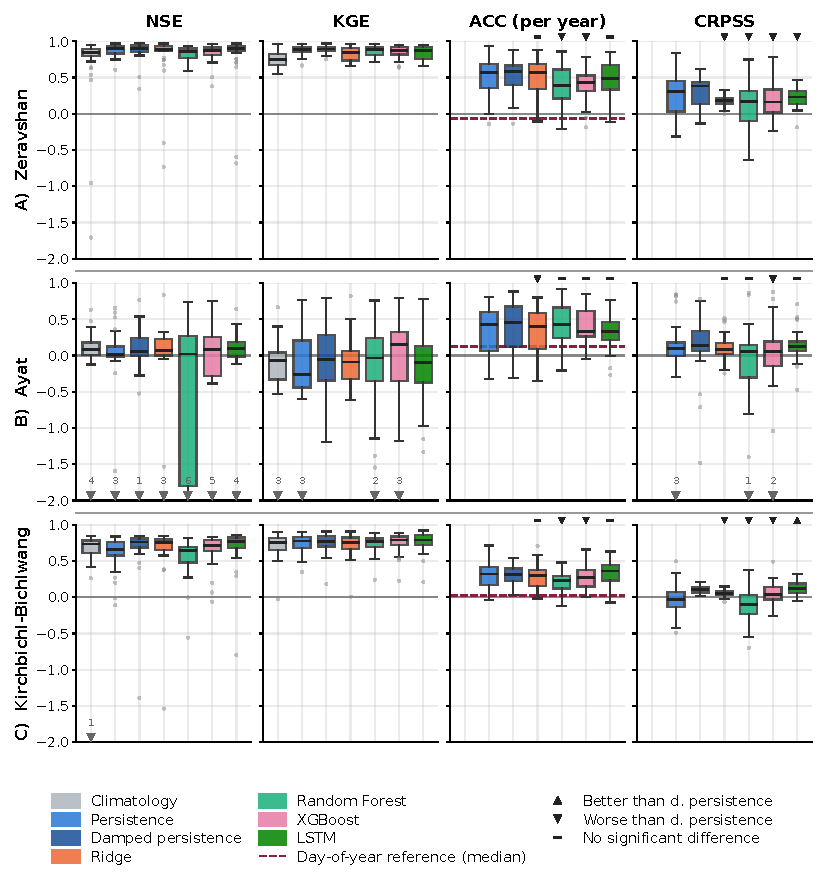
\includegraphics[width=\textwidth]{00_plots/fig03.pdf}
    \caption{LOGO-CV skill at short lead times, pooled over lead days 0--30. Rows are catchments (A: Zeravshan; B: Ayat; C: Kirchbichl--Bichlwang) and columns are metrics. Each box shows the distribution across cross-validation folds, one value per held-out hydrological year. ACC is computed within each fold. Grey triangles on the lower axis limit ($-2$) mark folds falling below it. The dashed line in the ACC column is the median of the day-of-year reference; ACC above it indicates skill beyond the seasonal cycle. Black symbols above the ACC and CRPSS boxes compare each learned model with damped persistence, using a paired bootstrap of the mean difference over hydrological years, with a Benjamini--Hochberg false discovery rate of 5\% applied across all catchments and models of each metric column.}
    \label{fig:box_short}
\end{figure}

\begin{figure}[H]
    \centering
    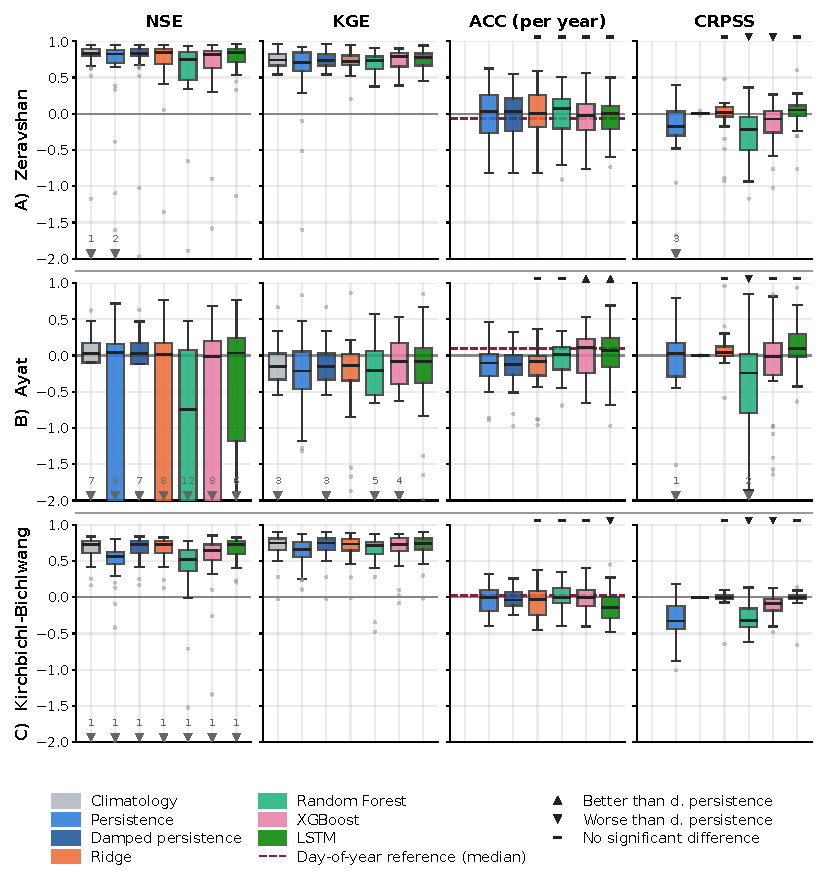
\includegraphics[width=\textwidth]{00_plots/fig04.pdf}
    \caption{LOGO-CV skill at long lead times, pooled over lead days 185--214. Rows are catchments (A: Zeravshan; B: Ayat; C: Kirchbichl--Bichlwang) and columns are metrics. Each box shows the distribution across cross-validation folds, one value per held-out hydrological year. ACC is computed within each fold. Grey triangles on the lower axis limit ($-2$) mark folds falling below it. The dashed line in the ACC column is the median of the day-of-year reference; ACC above it indicates skill beyond the seasonal cycle. Black symbols above the ACC and CRPSS boxes compare each learned model with damped persistence, using a paired bootstrap of the mean difference over hydrological years, with a Benjamini--Hochberg false discovery rate of 5\% applied across all catchments and models of each metric column.}
    \label{fig:box_long}
\end{figure}

Disaggregating ACC by initialisation month and lead bin (Figure~\ref{fig:heatmap}) resolves how anomaly skill decays with lead time. Because each cell pools anomalies across all test years, it also rewards differences in mean anomaly between years, so values are higher than the within-year ACC. Averaged over initialisation months, persistence decays monotonically at Zeravshan (0.85 to 0.22, levelling off beyond about 90~days) and Kirchbichl--Bichlwang (0.56 to 0.07) between the 0--14 and 151--215~day bins. At Ayat the rate of decay differs strongly between initialisation months: forecasts initialised from August to December retain an ACC of at least 0.41 in the last bin, whereas April initialisations lose all skill beyond 60~days. Within each catchment the learned models reproduce the patterns of the reference forecasts, which remain the best forecast in 61--77\% of cells. No learned model systematically exceeds damped persistence. Ridge tracks it most closely at all three catchments (mean absolute difference 0.03--0.05), sitting slightly below it at Zeravshan and Ayat and matching it on average at Kirchbichl--Bichlwang, while the LSTM follows it closely only at Ayat. The tree-based models depart furthest from it (0.09--0.22), and the LSTM at Kirchbichl--Bichlwang turns negative beyond 120~days.

\begin{figure}[H]
    \centering
    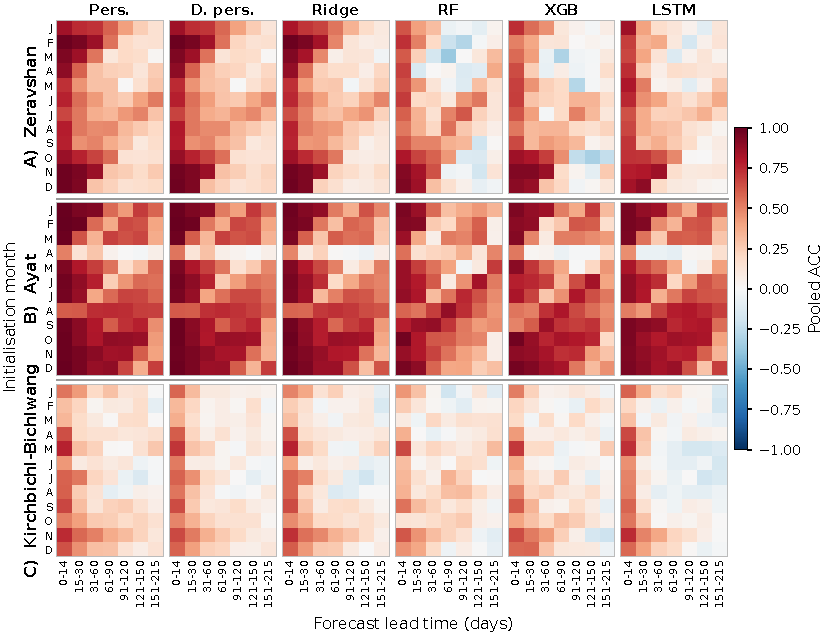
\includegraphics[width=\textwidth]{00_plots/fig05.pdf}
    \caption{Anomaly correlation coefficient by initialisation month (rows within each panel) and lead-time bin (columns within each panel, 0--14 to 151--215~days), for every catchment--model combination. Each cell pools the daily anomalies of all held-out test years for that initialisation month and lead bin. Unlike the per-fold ACC, pooled ACC includes differences in mean anomaly between years and is therefore generally higher.}
    \label{fig:heatmap}
\end{figure}

\subsection{Stage 2 - Hyperparameter Tuning}
\label{sec:results_st2}

Stage~2 asks whether the learned models can beat the reference forecasts once their hyperparameters are tuned. The corresponding figures for all nine catchments are given in \ref{app:stage2}. Figure~\ref{fig:configs} first shows how consistently the nested cross-validation selected a configuration: the mean rank of each of the 15 candidates across outer folds, the configuration winning most folds, and the spread in inner-CV ACC between configurations. LSTM configurations were largely interchangeable. Mean ranks clustered around the chance value of 8.0 (5.6--9.4 at Zeravshan, 5.1--11.6 at Ayat), and where the spread was wider, at Kirchbichl--Bichlwang (5.0--13.1), it was driven by poor configurations with the lowest learning rates rather than by a standout winner. The most frequently selected configuration won only 3/33 outer folds at Zeravshan (a seven-way tie), 5/29 at Ayat and 8/44 at Kirchbichl--Bichlwang, and the ACC range between best and worst configuration was only 0.021--0.039. Random Forest and XGBoost, in contrast, showed clear and stable preferences: mean ranks spanned nearly the full 1--15 scale, and single configurations dominated. Random Forest R08 won 32/33 outer folds at Zeravshan and all 29 at Ayat, and R02 won 41/44 at Kirchbichl--Bichlwang; XGBoost R09 won all 33 at Zeravshan and 24/44 at Kirchbichl--Bichlwang, and R01 won 26/29 at Ayat. The winners were consistently the more constrained configurations (Random Forest with a maximum depth of 10, XGBoost with a depth of 3), while the least constrained ranked last, including the Random Forest configuration closest to the library default used in Stage~1. The resulting differences in skill nonetheless remained small: the largest ACC range between configurations was 0.140 (XGBoost at Zeravshan), and at Kirchbichl--Bichlwang no model exceeded 0.048.

\begin{figure}[H]
    \centering
    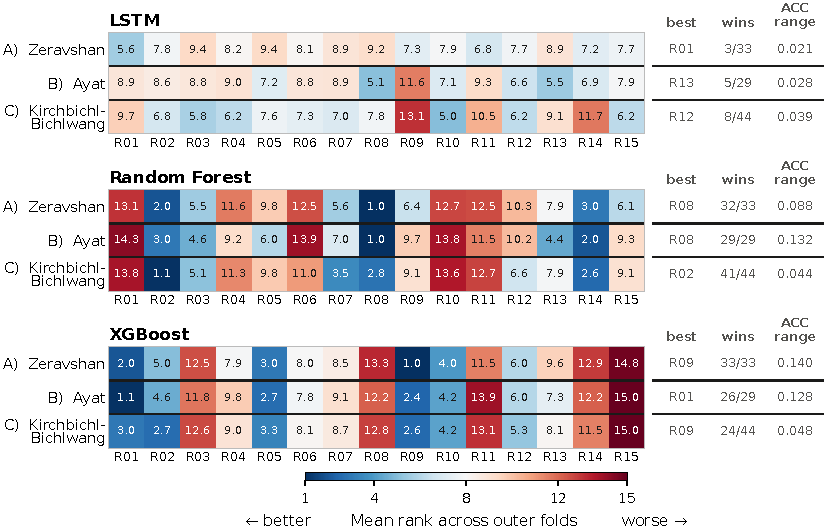
\includegraphics[width=\textwidth]{00_plots/fig06.pdf}
    \caption{Mean rank of the 15 candidate hyperparameter configurations across outer folds, by model (panels) and catchment (rows; A: Zeravshan; B: Ayat; C: Kirchbichl--Bichlwang). Configurations are ranked 1 (best inner-CV ACC) to 15 within each outer fold. Summary columns give the configuration with the most outright fold wins, its win count, and the best-to-worst spread in mean inner-CV ACC.}
    \label{fig:configs}
\end{figure}

Comparing each model's Stage~1 default with its tuned configuration (Figures~\ref{fig:tune_short} and~\ref{fig:tune_long}) shows that tuning helped the tree ensembles but not the LSTM. At 0--30~days tuning raised the median ACC of Random Forest and XGBoost at every catchment (by 0.02--0.14 and 0.07--0.15) and their median CRPSS (by 0.11--0.19 and 0.04--0.17), while the LSTM's medians changed by at most 0.05, as its flat configuration ranking anticipated. These gains narrowed the gap between the learned models and damped persistence, however still no tuned model clearly surpassed damped persistence. At Zeravshan damped persistence kept the highest median ACC (0.58 against 0.53 for tuned Random Forest and XGBoost) and CRPSS (0.38 against 0.28), with tuned XGBoost and the LSTM significantly worse on CRPSS. At Ayat tuned Random Forest and XGBoost matched or exceeded it on median ACC (0.45 and 0.49 against 0.45) and CRPSS (0.22 against 0.14), and at Kirchbichl--Bichlwang all three tuned models slightly exceeded its median ACC (0.33--0.34 against 0.32), but none of these differences was significant according to the paired bootstrap. At 185--214~days median ACC stayed within $\pm0.12$ of zero for every tuned model. Tuned Random Forest and XGBoost were significantly better than damped persistence at Ayat (0.12 and 0.11), though mainly because damped persistence fell to $-0.12$ there, and tuning lifted the LSTM at Kirchbichl--Bichlwang from $-0.14$ to $-0.05$, removing its Stage~1 deficit. On CRPSS, tuning closed the deficits of the tree ensembles onto zero at Zeravshan and Kirchbichl--Bichlwang (Random Forest $-0.22\rightarrow0.04$ and $-0.31\rightarrow-0.01$). With damped persistence identical to climatology at this lead, the tuned models therefore matched the reference rather than beat it, except at Ayat, where all three sat above it (0.14--0.15), significantly so only for the LSTM. NSE and KGE stayed catchment-controlled at both leads.

\begin{figure}[H]
    \centering
    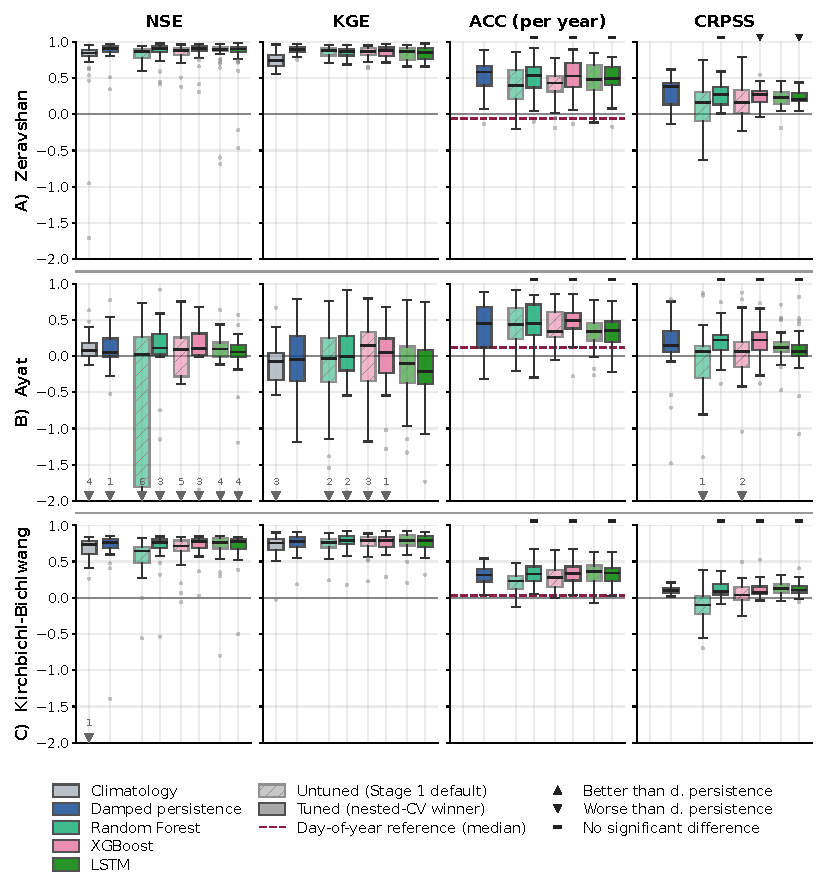
\includegraphics[width=\textwidth]{00_plots/fig07.pdf}
    \caption{Effect of hyperparameter tuning on LOGO-CV skill at short lead times, pooled over lead days 0--30. Rows are catchments (A: Zeravshan; B: Ayat; C: Kirchbichl--Bichlwang) and columns are metrics. Each learned model is shown as a pair: its default configuration (hatched) beside the configuration selected by nested cross-validation in each outer fold (solid). Each box shows the distribution across cross-validation folds, one value per held-out hydrological year. ACC is computed within each fold. Grey triangles on the lower axis limit ($-2$) mark folds falling below it. The dashed line in the ACC column is the median of the day-of-year reference; ACC above it indicates skill beyond the seasonal cycle. Black symbols above the tuned ACC and CRPSS boxes compare each tuned model with damped persistence, using a paired bootstrap of the mean difference over hydrological years, with a Benjamini--Hochberg false discovery rate of 5\% applied across all catchments and models of each metric column.}
    \label{fig:tune_short}
\end{figure}

\begin{figure}[H]
    \centering
    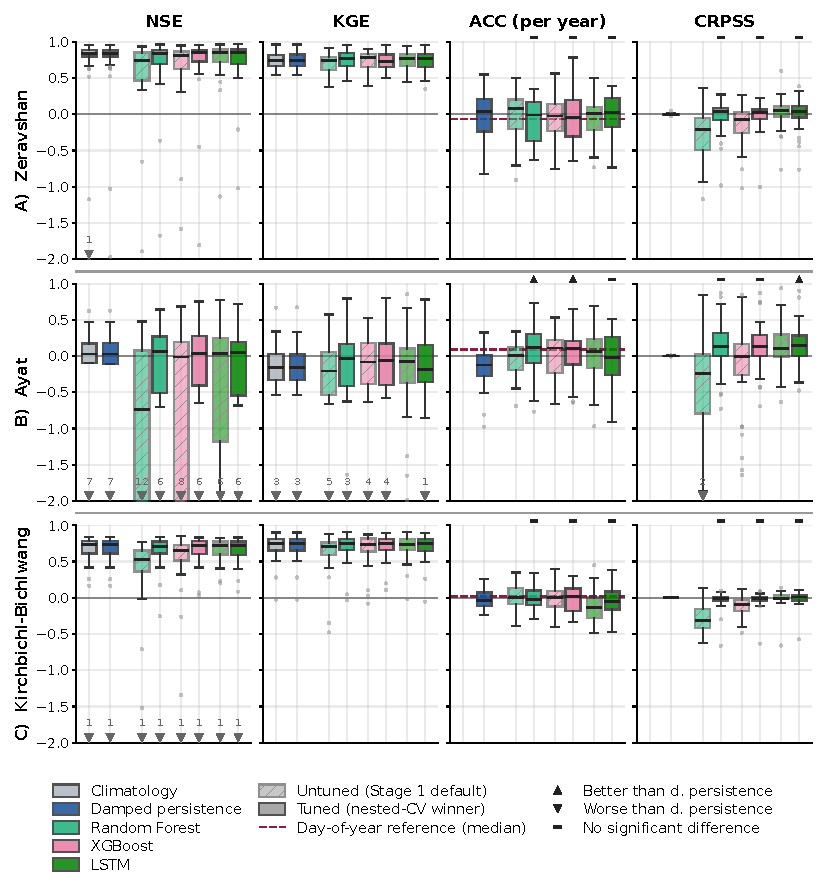
\includegraphics[width=\textwidth]{00_plots/fig08.pdf}
    \caption{Effect of hyperparameter tuning on LOGO-CV skill at long lead times, pooled over lead days 185--214. Rows are catchments (A: Zeravshan; B: Ayat; C: Kirchbichl--Bichlwang) and columns are metrics. Each learned model is shown as a pair: its default configuration (hatched) beside the configuration selected by nested cross-validation in each outer fold (solid). Each box shows the distribution across cross-validation folds, one value per held-out hydrological year. ACC is computed within each fold. Grey triangles on the lower axis limit ($-2$) mark folds falling below it. The dashed line in the ACC column is the median of the day-of-year reference; ACC above it indicates skill beyond the seasonal cycle. Black symbols above the tuned ACC and CRPSS boxes compare each tuned model with damped persistence, using a paired bootstrap of the mean difference over hydrological years, with a Benjamini--Hochberg false discovery rate of 5\% applied across all catchments and models of each metric column.}
    \label{fig:tune_long}
\end{figure}

\subsection{Stage 3 - Sensitivity Test}
\label{sec:results_st3}

Stage~3 tests how much the models rely on the meteorological forcing at inference time. The same metrics are reported for every catchment and model, but as the per-fold difference between the scores obtained with the original and with the corrupted forcing, over the full forecast horizon (Figure~\ref{fig:sensitivity}). The corresponding figures for all nine catchments are given in \ref{app:stage3}. Replacing the original forcing with a donor year's had a negligible effect throughout. Across all four models, four metrics and three catchments, every median difference fell between $-0.001$ and $0.012$, and the share of folds in which corruption reduced skill ranged from 42\% to 71\%, against the 50\% expected of forcing that carries no information. Ridge changed least, its fold spread being the narrowest of the four models in every metric at Zeravshan and Ayat (interquartile ranges of 0.001--0.006). At Kirchbichl--Bichlwang XGBoost was the least affected model, with interquartile ranges of at most 0.001 and median changes of zero, whereas at Ayat the two tree ensembles behaved much alike (0.010--0.033). The LSTM changed the most, with interquartile ranges of 0.006--0.097, widest on ACC at Kirchbichl--Bichlwang (0.097) and Zeravshan (0.039). The most consistent effects were those on the LSTM at Kirchbichl--Bichlwang and on Random Forest at Ayat, where corruption reduced skill in 61--68\% and 61--71\% of folds on every metric, yet even there the median changes stayed at or below 0.012.

\begin{figure}[H]
    \centering
    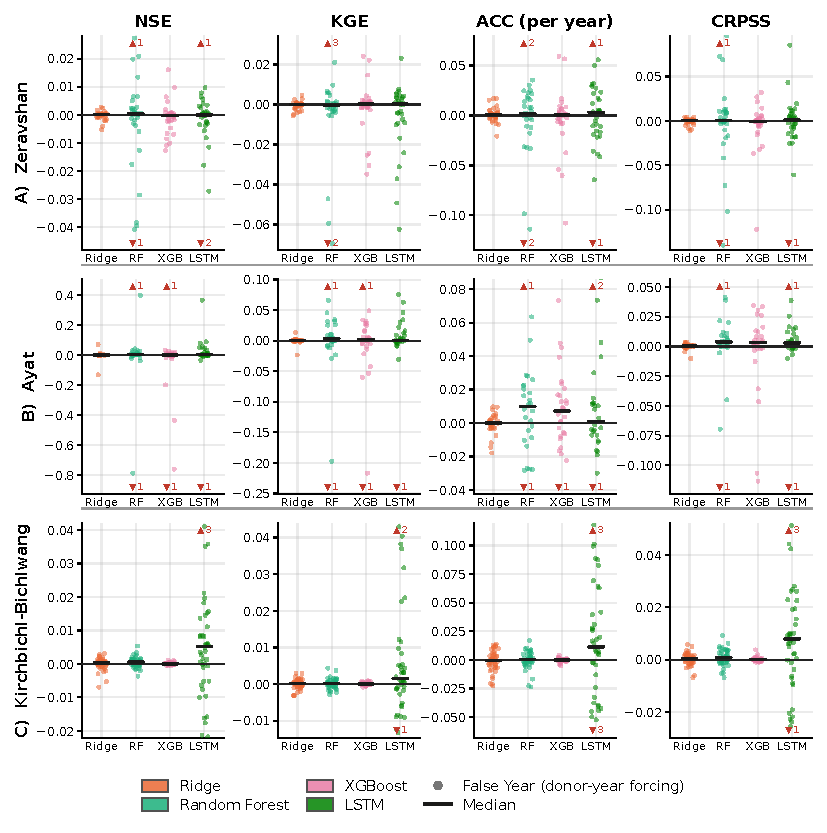
\includegraphics[width=\textwidth]{00_plots/fig09.pdf}
    \caption{Sensitivity of each learned model to its meteorological forcing, scored over the full forecast horizon (lead days 0--214). Each point is the difference between the two scores, so positive values denote skill lost when the forcing is corrupted and values near zero denote a model insensitive to its forcing. Rows are catchments (A: Zeravshan; B: Ayat; C: Kirchbichl--Bichlwang), columns are metrics, and each panel holds one strip per model with one point per fold and a marker at the median. ACC is computed within each fold. Triangles at the upper and lower panel edges mark folds falling outside the axis range.}
    \label{fig:sensitivity}
\end{figure}


\section{Discussion}
\label{sec:discussion}

In data-scarce regions such as Central Asia, developing accurate discharge forecasting tools from freely available data, such as ECMWF's SEAS5 seasonal climate forecasts, could be a valuable aid to river management. In nival--glacial-dominated catchments, however, the main obstacle to seasonal discharge prediction is the dominance of the seasonal cycle: it accounts for most of the discharge variance, so any forecast that follows climatology closely will inevitably score well on volumetric metrics such as NSE or KGE \citep{ruzzante2026}. Our strategy for avoiding this problem was to work in anomaly space, training the models to predict a log-transformed anomaly rather than raw discharge, so that they could not simply reproduce climatology. The models were likewise supplied with the log-transformed anomaly at the initialisation date rather than the raw discharge, so that raw discharge never entered as a feature. Even after hyperparameter tuning, however, this approach did not produce models that consistently beat damped persistence in either lead-time window.

Removing the seasonal cycle from the target did not by itself produce skill beyond persistence, in either the Central Asian or the European mountain catchment. At 0--30~days every forecast, climatology included, reached median NSE values of 0.85--0.91 at Zeravshan and 0.65--0.77 at Kirchbichl--Bichlwang, yet on ACC and CRPSS no learned model was significantly better than damped persistence, with a single exception: the CRPSS of the LSTM at Kirchbichl--Bichlwang (0.13 against 0.11). At long lead times the within-year ACC of every forecast converged towards zero. This outcome parallels the North American single-catchment hybrid study of \citet{swiftlapointe2025}, in which no SEAS5-forced LSTM configuration outperformed a climatology-forced reference and a daily-resolution model reached an NSE of 0.9 while carrying essentially no interannual anomaly information. Our results show that the problem is not confined to models trained on raw discharge, and that it persists across nival--glacial-dominated catchments in different regions, here Europe and Central Asia.

The steppe regime fails in a different way. At Ayat the seasonal cycle explains almost none of the discharge variance (median NSE of climatology 0.08), so anomaly skill is not masked by it, and yet that skill was carried by persistence rather than by the learned models. At 0--30~days damped persistence reached a median ACC of 0.45, which no learned model exceeded significantly. The learned models were significantly better than damped persistence only at 185--214~days, where XGBoost and the LSTM reached median ACCs of 0.11 and 0.07 against $-0.12$. These gains reflect the loss of skill of damped persistence rather than a usable signal in the models, which did not clearly exceed the day-of-year reference (0.10). Moreover, no forecast retained usable volumetric accuracy, with median NSE between $-0.74$ and 0.10 across both windows. Ayat thus shows the most interannual predictability of the catchments tested, but that predictability appears to reside in the antecedent discharge anomaly, which persistence already exploits, rather than in anything the learned models add.

Stage~2 showed that, at least within the hyperparameter space explored here, the skill ceiling was not found in the models themselves. The configuration search behaved differently across architectures: the LSTM was largely indifferent to it, whereas Random Forest and XGBoost consistently selected their most constrained configurations, rather than the deeper, less regularised library defaults used in Stage~1. Tuning thus mainly corrected the overfitting of the untuned tree ensembles: it narrowed their gap to damped persistence at short lead and lifted their long-lead CRPSS from well below zero to or above the climatological reference, but did not carry them beyond damped persistence. At the two nival--glacial-dominated catchments no tuned model significantly exceeded it, and at Ayat they did so only at 185--214~days, where damped persistence had itself lost its skill. We therefore argue that the limiting factor lies in the seasonal forcing, which we later test directly in Stage~3. The issue is clearest when the forcing is viewed against the size of the catchments: SEAS5 is supplied on a $1^\circ\times1^\circ$ grid (roughly $111\times76$~km per cell at these latitudes), and the models receive a cosine-weighted mean over a box of 2 to 12 such cells enclosing each catchment (Table~\ref{tab:catchments}). The orographic precipitation and snowpack gradients that drive discharge vary over much shorter distances and are averaged away before any model sees them.

Stage~3 confirms that the climate forcing contributes little information to the models. Replacing the forcing with that of a donor year changed almost nothing: every median difference stayed at or below 0.012, regardless of model or catchment. The few consistent effects, on the LSTM at Kirchbichl--Bichlwang and on Random Forest at Ayat, show that the forcing was not ignored entirely, but they are too small to account for any meaningful share of the models' skill. Because the corrupted runs kept the seasonal encodings and the antecedent discharge anomaly unchanged, the models must rely almost entirely on these inputs. This explains why they could at best match the persistence references: both draw their information from the same antecedent anomaly.

Few freely available seasonal forecast products are currently an alternative to SEAS5 in Central Asia, and together with the scarcity of discharge and station observations, data availability remains the main limitation for developing seasonal discharge forecasts in the region. Within SEAS5 itself, the spatial averaging used here is a point to revisit: supplying the models with forcing downscaled to the catchment might preserve some of the orographic gradients that the box mean removes. Another way of using SEAS5 that was not tested here is the aggregation strategy of \citet{swiftlapointe2025}, who recovered interannual skill by aggregating to monthly resolution and predicting at monthly intervals, at the cost of temporal detail.

A second approach not tested in this study, but with the potential to improve performance, is training across multiple catchments rather than one catchment at a time. This has been done in North America both with a conventional multi-catchment LSTM \citep{kratzert2019} and with the ``Hydra-LSTM'' variant \citep{ruparell2025}, which is trained on several catchments and then applied to catchments it has never seen. Training such a model on separate data-rich catchments and transferring it to the data-scarce Central Asian ones may be one way of overcoming the data limitations encountered in the region.

For operational seasonal forecasting in Central Asia, the practical implication is that damped persistence remains the benchmark to beat: none of the configurations tested here significantly outperformed it in the nival--glacial-dominated catchments, and in the steppe catchment they did so only once the reference itself had lost its skill. This also has consequences for how such forecasts are evaluated: in regimes where the seasonal cycle dominates the variance, a high NSE or KGE can be reached by climatology alone, and reporting these metrics alone overstates what a forecast can actually deliver. Anomaly-based scores such as ACC and CRPSS, assessed against a persistence reference rather than against climatology, are the more honest measure of whether a model carries interannual information.

\section{Conclusions}
\label{sec:conclusions}

\begin{itemize}
\item After testing multiple model architectures and training in log-transformed anomaly space, none of the models were able to significantly outperform the damped persistence reference in the nival--glacial-dominated Central Asian catchments.
\item The steppe regime fails in a different way: its anomaly skill was carried by persistence, the models exceeded damped persistence only at long lead times once the reference itself had lost its skill, and their volumetric accuracy collapsed, leaving them equally unusable in an operational setting.
\item The skill ceiling lies upstream, in the SEAS5 forcing as used here. Replacing it with the forcing of a donor year changed median scores by at most 0.012, so the models relied almost entirely on the antecedent discharge anomaly. Averaged over $1^\circ$ cells spanning several times the catchment area, the forcing may be too coarse to resolve the orographic gradients that drive discharge; we therefore recommend testing finer representations of it, such as downscaled forecasts.
\item In regimes dominated by the seasonal cycle, high NSE or KGE can be reached by climatology alone; anomaly-based scores assessed against a persistence reference are the more honest measure of forecast skill.
\end{itemize}

\section*{CRediT authorship contribution statement}

\textbf{Diegopablo Pineda Schwarz:} Conceptualization, Formal analysis, Investigation, Methodology, Software, Visualization, Writing -- original draft, Writing -- review \& editing. \textbf{Iulii Didovets:} Conceptualization, Methodology, Project administration, Resources, Supervision, Writing -- review \& editing. \textbf{Bijan Fallah:} Conceptualization, Methodology, Software, Supervision, Validation, Writing -- review \& editing. \textbf{Tursyn Tillakarim:} Conceptualization, Resources, Data curation.

\section*{Declaration of competing interest}

The authors report no declarations of interest.

\section*{Data availability}

The code used in this study, covering the SEAS5 download and preprocessing, all three experimental stages and the reproduction of every figure, is openly available on Zenodo under the MIT licence \citep{pinedaschwarz2026code}. SEAS5 seasonal forecasts are freely available from the Copernicus Climate Data Store \citep{copernicus2018}. Discharge observations for the European catchments are available from the Global Runoff Data Centre \citep{grdc2026}. Discharge observations for the Central Asian catchments were provided by Kazhydromet and Tajik Hydromet and are not publicly available.

\section*{Acknowledgements}

The authors thank the German Federal Ministry of Education and Research and the State of Brandenburg for supporting this project by providing resources on the high-performance computer system at the Potsdam Institute for Climate Impact Research. 
The contribution of Bijan Fallah was funded by the Deutsche Forschungsgemeinschaft (DFG, German Research Foundation) within the AMOC-Millennia project (grant no.~550037087).

This research would not have been possible without the observed discharge data collected and provided by the Agency for Hydrometeorology of the Republic of Kazakhstan (Kazhydromet) and the Agency for Hydrometeorology of the Republic of Tajikistan (Tajik Hydromet). We are particularly grateful to Safarkhon Sharofiddinov, Head of the Hydrological Forecasting Department at the Agency for Hydrometeorology of the Republic of Tajikistan, for making the Tajik discharge records available.

\section*{Declaration of generative AI and AI-assisted technologies in the manuscript preparation process}

During the preparation of this work the authors used Claude (Anthropic), in order to assist with writing and debugging the code of the modelling and evaluation pipeline, and with reviewing and editing the manuscript text. After using this tool, the authors reviewed and edited the content as needed and take full responsibility for the content of the published article.


\appendix

\section{Stage 1 results for all catchments}
\label{app:stage1}
\setcounter{figure}{0}

This appendix extends Section~\ref{sec:results_st1} to all nine study catchments. Each main-text figure is repeated once per hydrological regime: the Central Asian nival--glacial-dominated mountain catchments (Zeravshan, Ulken Boken, Kurshim), the Central Asian nival-dominated steppe catchments (Kalkutan, Esil, Ayat, Zhabay), and the European nival--glacial-dominated mountain catchments (Kirchbichl--Bichlwang, Diepoldsau--Rietbr\"ucke). Figures~\ref{fig:appA_short_mountain}--\ref{fig:appA_short_europe} show the LOGO-CV skill of the four learned models and the three reference forecasts pooled over lead days 0--30, Figures~\ref{fig:appA_long_mountain}--\ref{fig:appA_long_europe} the same pooled over lead days 185--214, and Figures~\ref{fig:appA_heatmap_mountain}--\ref{fig:appA_heatmap_europe} the pooled ACC by initialisation month and lead-time bin. Metrics, symbols and significance tests are as described for Figures~\ref{fig:box_short}--\ref{fig:heatmap}.

\begin{figure}[!htbp]
    \centering
    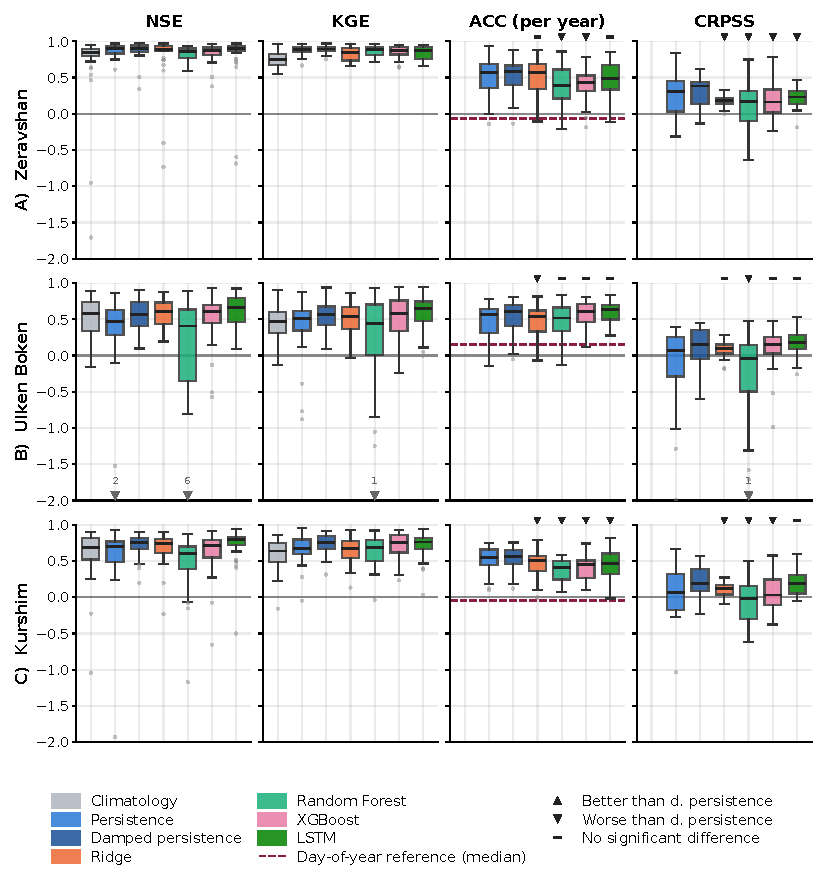
\includegraphics[width=\textwidth]{00_appendix/figA01.pdf}
    \caption{As Figure~\ref{fig:box_short} (LOGO-CV skill pooled over lead days 0--30), for the Central Asian nival--glacial-dominated mountain catchments (A: Zeravshan; B: Ulken Boken; C: Kurshim).}
    \label{fig:appA_short_mountain}
\end{figure}

\begin{figure}[!htbp]
    \centering
    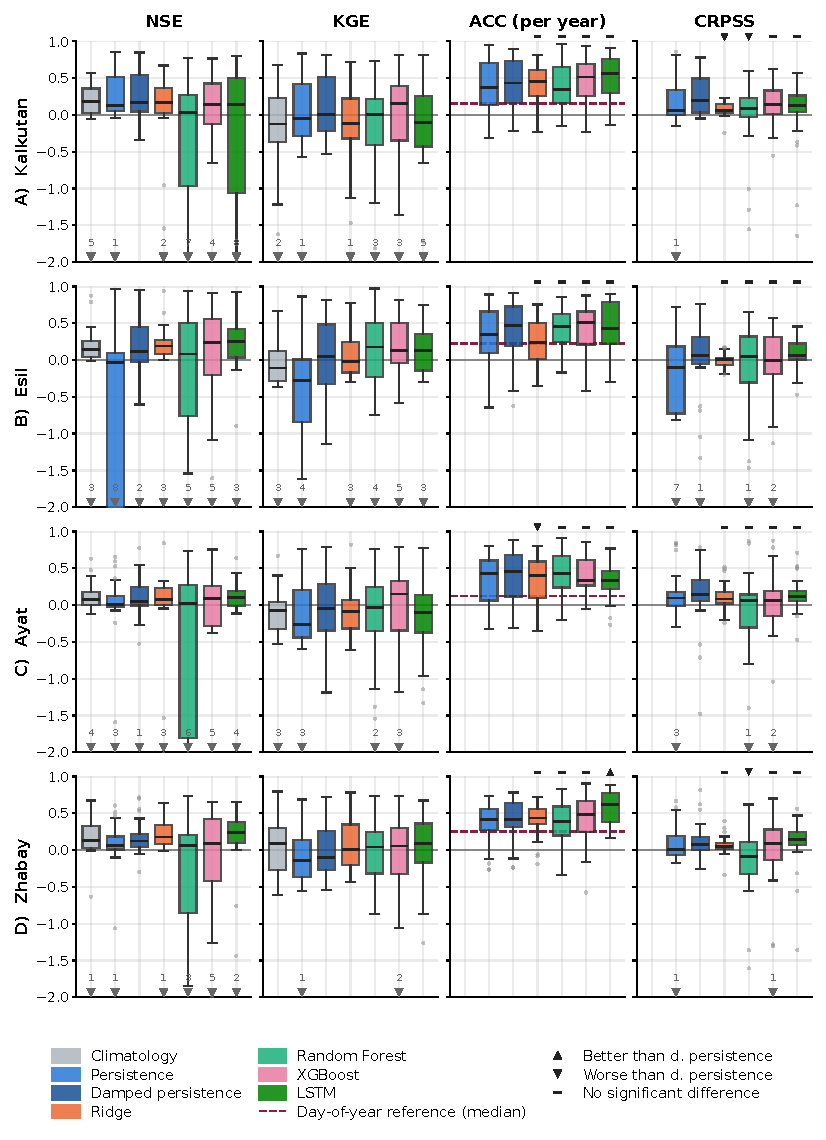
\includegraphics[width=\textwidth,height=0.8\textheight,keepaspectratio]{00_appendix/figA02.pdf}
    \caption{As Figure~\ref{fig:box_short} (LOGO-CV skill pooled over lead days 0--30), for the Central Asian nival-dominated steppe catchments (A: Kalkutan; B: Esil; C: Ayat; D: Zhabay).}
    \label{fig:appA_short_steppe}
\end{figure}

\begin{figure}[!htbp]
    \centering
    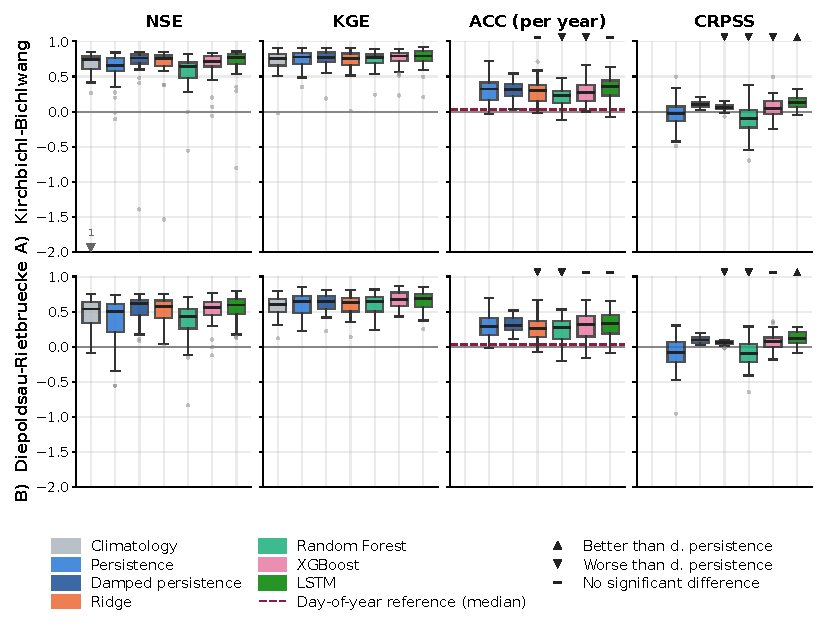
\includegraphics[width=\textwidth]{00_appendix/figA03.pdf}
    \caption{As Figure~\ref{fig:box_short} (LOGO-CV skill pooled over lead days 0--30), for the European nival--glacial-dominated mountain catchments (A: Kirchbichl--Bichlwang; B: Diepoldsau--Rietbr\"ucke).}
    \label{fig:appA_short_europe}
\end{figure}

\begin{figure}[!htbp]
    \centering
    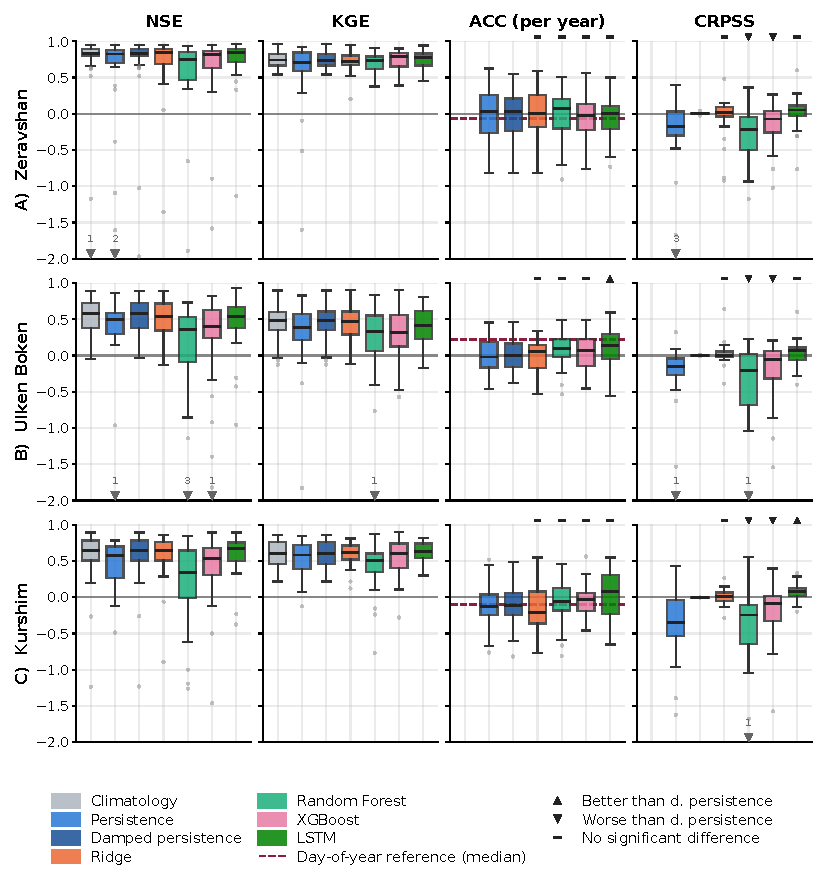
\includegraphics[width=\textwidth]{00_appendix/figA04.pdf}
    \caption{As Figure~\ref{fig:box_long} (LOGO-CV skill pooled over lead days 185--214), for the Central Asian nival--glacial-dominated mountain catchments (A: Zeravshan; B: Ulken Boken; C: Kurshim).}
    \label{fig:appA_long_mountain}
\end{figure}

\begin{figure}[!htbp]
    \centering
    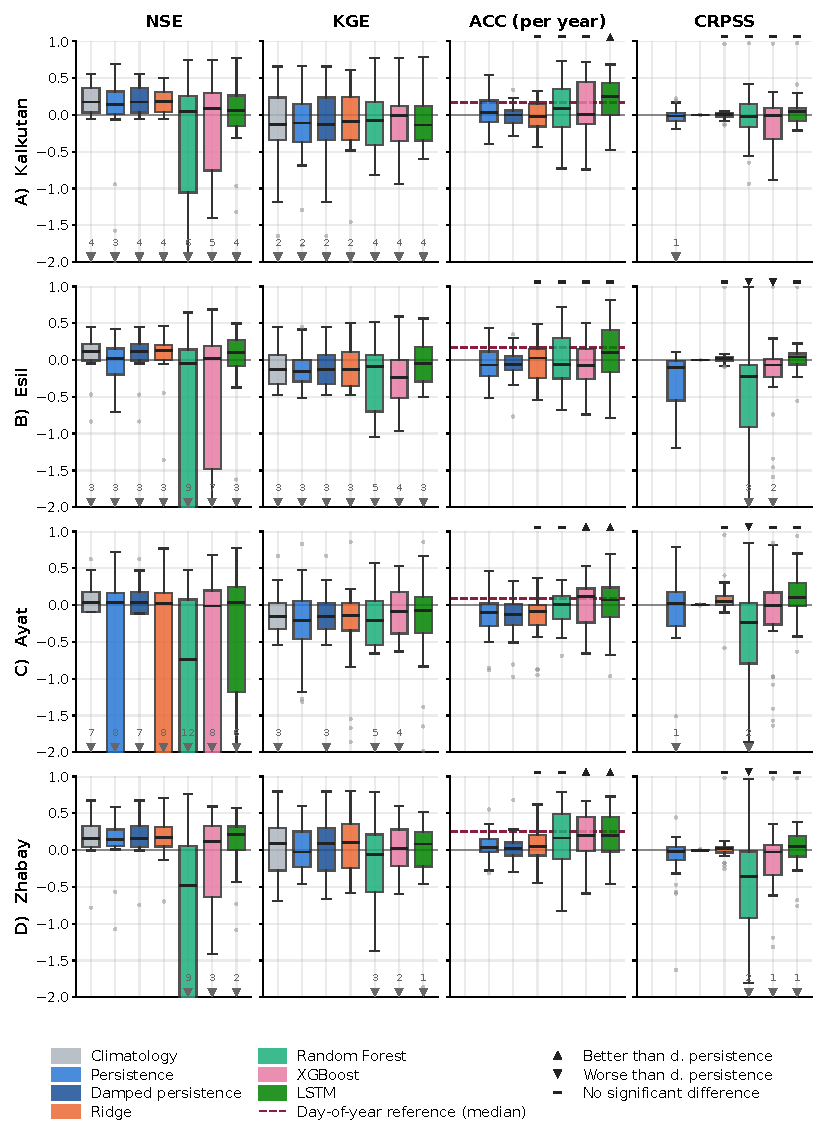
\includegraphics[width=\textwidth,height=0.8\textheight,keepaspectratio]{00_appendix/figA05.pdf}
    \caption{As Figure~\ref{fig:box_long} (LOGO-CV skill pooled over lead days 185--214), for the Central Asian nival-dominated steppe catchments (A: Kalkutan; B: Esil; C: Ayat; D: Zhabay).}
    \label{fig:appA_long_steppe}
\end{figure}

\begin{figure}[!htbp]
    \centering
    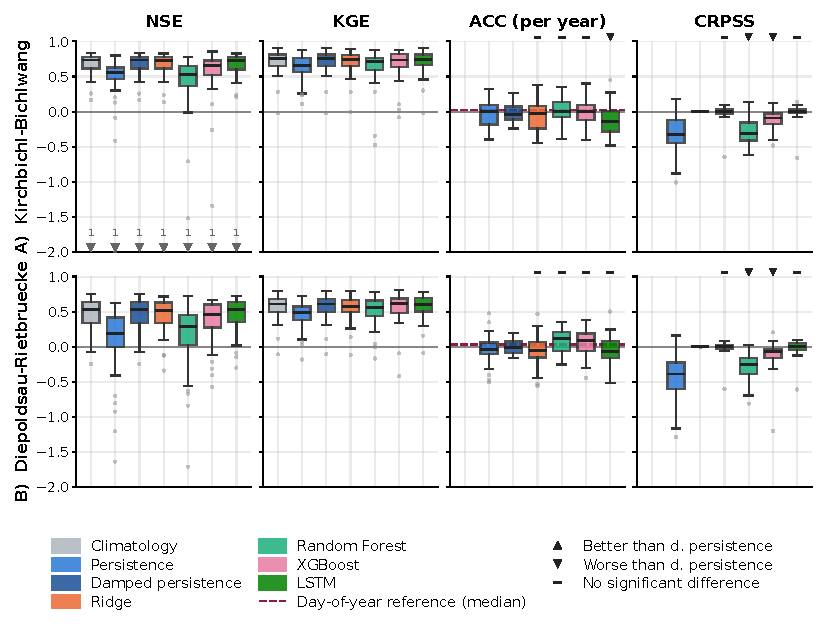
\includegraphics[width=\textwidth]{00_appendix/figA06.pdf}
    \caption{As Figure~\ref{fig:box_long} (LOGO-CV skill pooled over lead days 185--214), for the European nival--glacial-dominated mountain catchments (A: Kirchbichl--Bichlwang; B: Diepoldsau--Rietbr\"ucke).}
    \label{fig:appA_long_europe}
\end{figure}

\begin{figure}[!htbp]
    \centering
    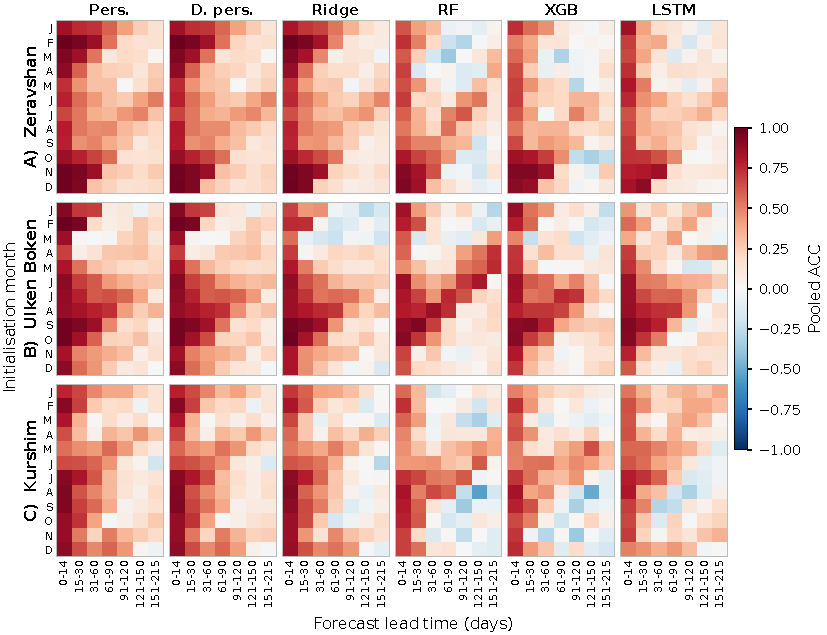
\includegraphics[width=\textwidth]{00_appendix/figA07.pdf}
    \caption{As Figure~\ref{fig:heatmap} (pooled ACC by initialisation month and lead-time bin), for the Central Asian nival--glacial-dominated mountain catchments (A: Zeravshan; B: Ulken Boken; C: Kurshim).}
    \label{fig:appA_heatmap_mountain}
\end{figure}

\begin{figure}[!htbp]
    \centering
    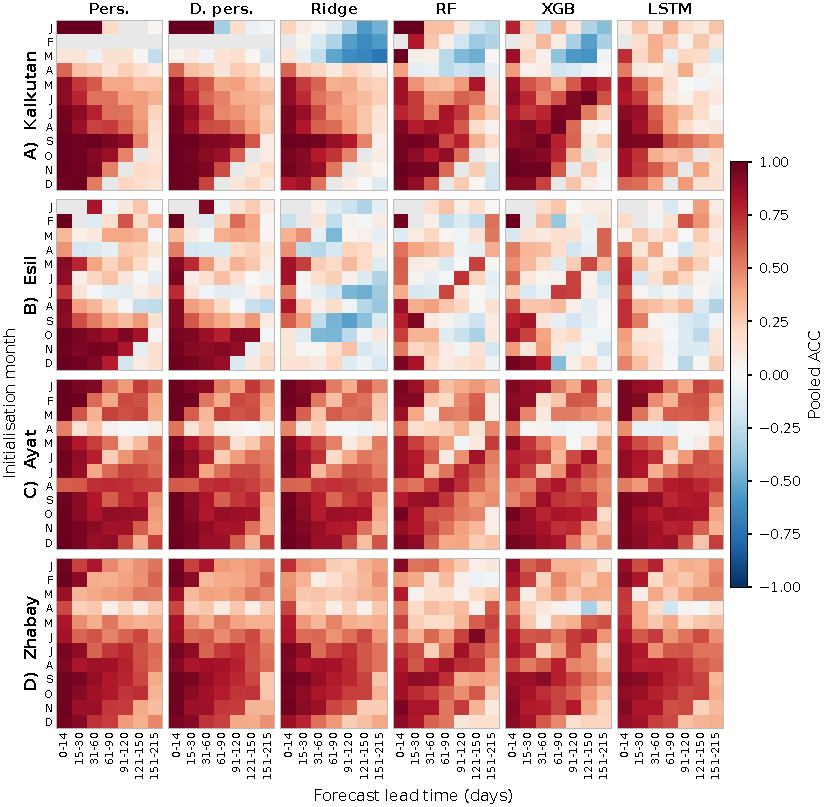
\includegraphics[width=\textwidth]{00_appendix/figA08.pdf}
    \caption{As Figure~\ref{fig:heatmap} (pooled ACC by initialisation month and lead-time bin), for the Central Asian nival-dominated steppe catchments (A: Kalkutan; B: Esil; C: Ayat; D: Zhabay).}
    \label{fig:appA_heatmap_steppe}
\end{figure}

\begin{figure}[!htbp]
    \centering
    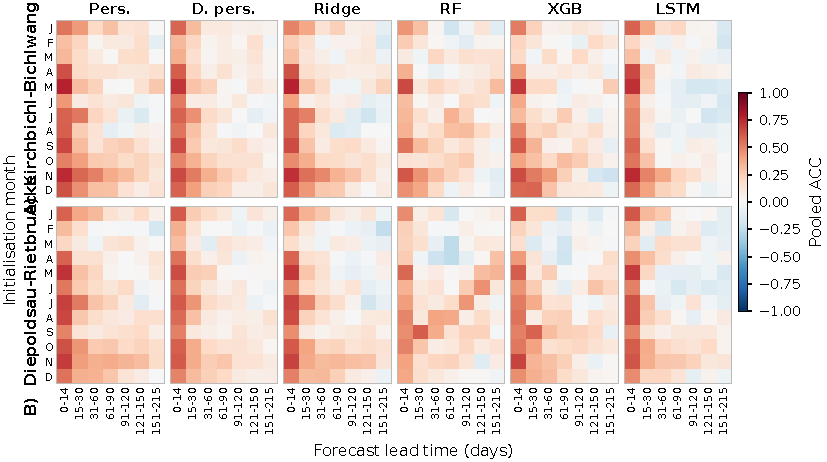
\includegraphics[width=\textwidth]{00_appendix/figA09.pdf}
    \caption{As Figure~\ref{fig:heatmap} (pooled ACC by initialisation month and lead-time bin), for the European nival--glacial-dominated mountain catchments (A: Kirchbichl--Bichlwang; B: Diepoldsau--Rietbr\"ucke).}
    \label{fig:appA_heatmap_europe}
\end{figure}

\clearpage

\section{Stage 2 results for all catchments}
\label{app:stage2}
\setcounter{figure}{0}

This appendix extends Section~\ref{sec:results_st2} to all nine study catchments. Each main-text figure is repeated once per hydrological regime: the Central Asian nival--glacial-dominated mountain catchments (Zeravshan, Ulken Boken, Kurshim), the Central Asian nival-dominated steppe catchments (Kalkutan, Esil, Ayat, Zhabay), and the European nival--glacial-dominated mountain catchments (Kirchbichl--Bichlwang, Diepoldsau--Rietbr\"ucke). Figures~\ref{fig:appB_configs_mountain}--\ref{fig:appB_configs_europe} show the mean rank of the 15 candidate hyperparameter configurations of each tuned model across outer folds, together with the configuration winning the most outer folds, its number of wins, and the best-to-worst spread in mean inner-CV ACC. Figures~\ref{fig:appB_short_mountain}--\ref{fig:appB_short_europe} and~\ref{fig:appB_long_mountain}--\ref{fig:appB_long_europe} compare the untuned Stage~1 configuration of Random Forest, XGBoost and the LSTM with the configuration selected by nested cross-validation, beside climatology and damped persistence, pooled over lead days 0--30 and 185--214, respectively. Metrics, symbols and significance tests are as described for Figures~\ref{fig:configs}--\ref{fig:tune_long}.

\begin{figure}[!htbp]
    \centering
    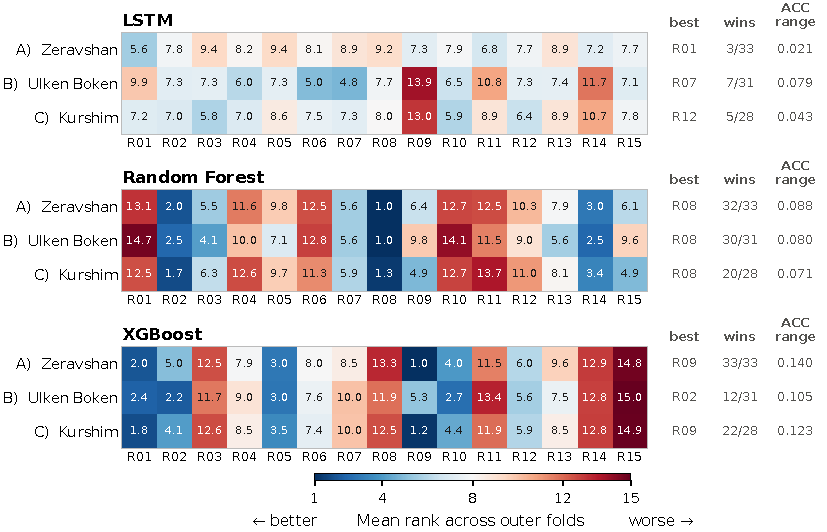
\includegraphics[width=\textwidth]{00_appendix/figB01.pdf}
    \caption{As Figure~\ref{fig:configs} (mean rank of the 15 candidate hyperparameter configurations across outer folds), for the Central Asian nival--glacial-dominated mountain catchments (A: Zeravshan; B: Ulken Boken; C: Kurshim).}
    \label{fig:appB_configs_mountain}
\end{figure}

\begin{figure}[!htbp]
    \centering
    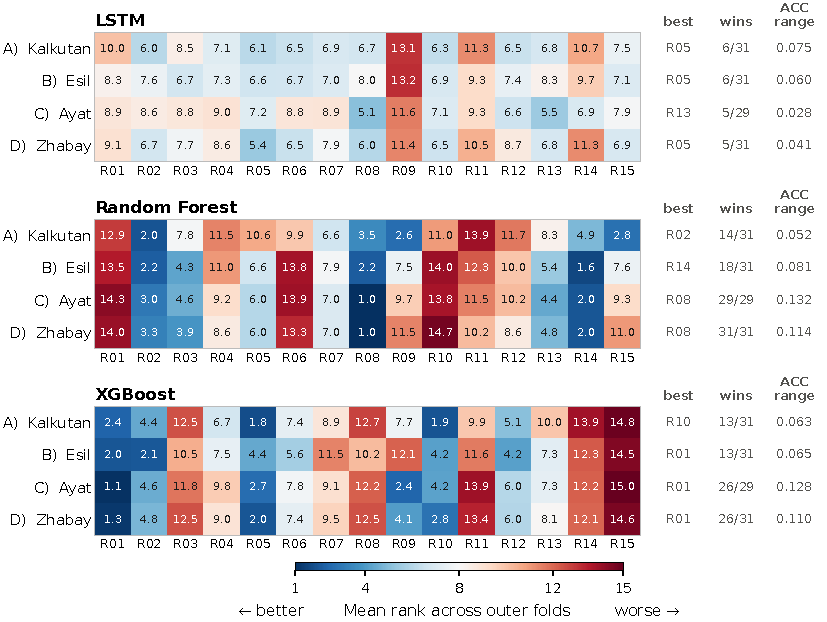
\includegraphics[width=\textwidth]{00_appendix/figB02.pdf}
    \caption{As Figure~\ref{fig:configs} (mean rank of the 15 candidate hyperparameter configurations across outer folds), for the Central Asian nival-dominated steppe catchments (A: Kalkutan; B: Esil; C: Ayat; D: Zhabay).}
    \label{fig:appB_configs_steppe}
\end{figure}

\begin{figure}[!htbp]
    \centering
    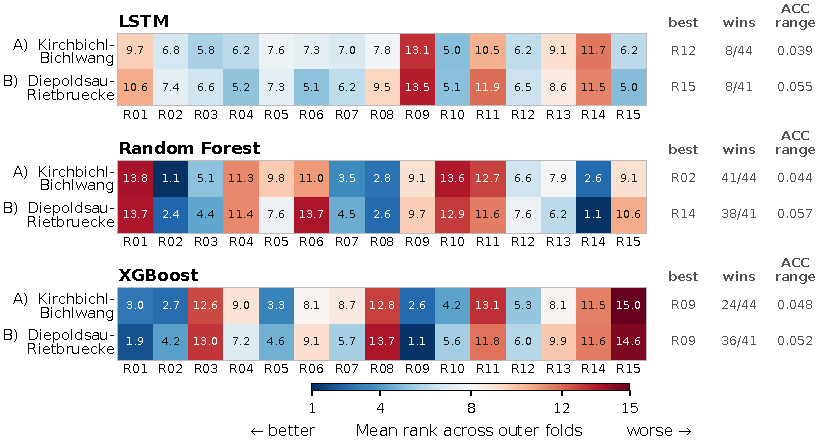
\includegraphics[width=\textwidth]{00_appendix/figB03.pdf}
    \caption{As Figure~\ref{fig:configs} (mean rank of the 15 candidate hyperparameter configurations across outer folds), for the European nival--glacial-dominated mountain catchments (A: Kirchbichl--Bichlwang; B: Diepoldsau--Rietbr\"ucke).}
    \label{fig:appB_configs_europe}
\end{figure}

\begin{figure}[!htbp]
    \centering
    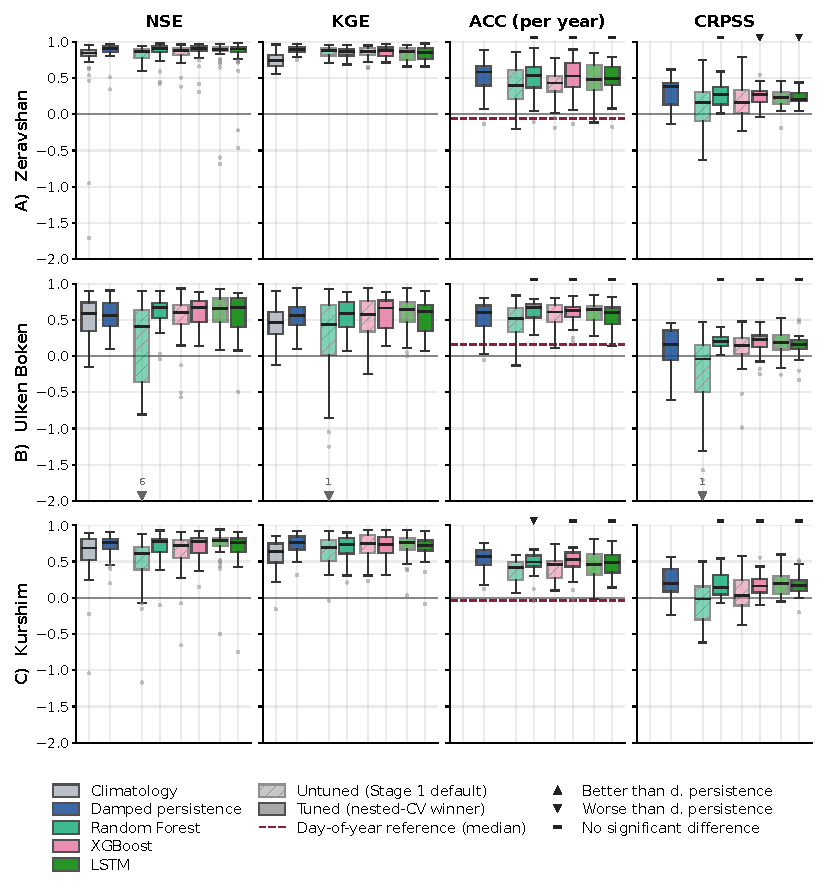
\includegraphics[width=\textwidth]{00_appendix/figB04.pdf}
    \caption{As Figure~\ref{fig:tune_short} (effect of hyperparameter tuning, pooled over lead days 0--30), for the Central Asian nival--glacial-dominated mountain catchments (A: Zeravshan; B: Ulken Boken; C: Kurshim).}
    \label{fig:appB_short_mountain}
\end{figure}

\begin{figure}[!htbp]
    \centering
    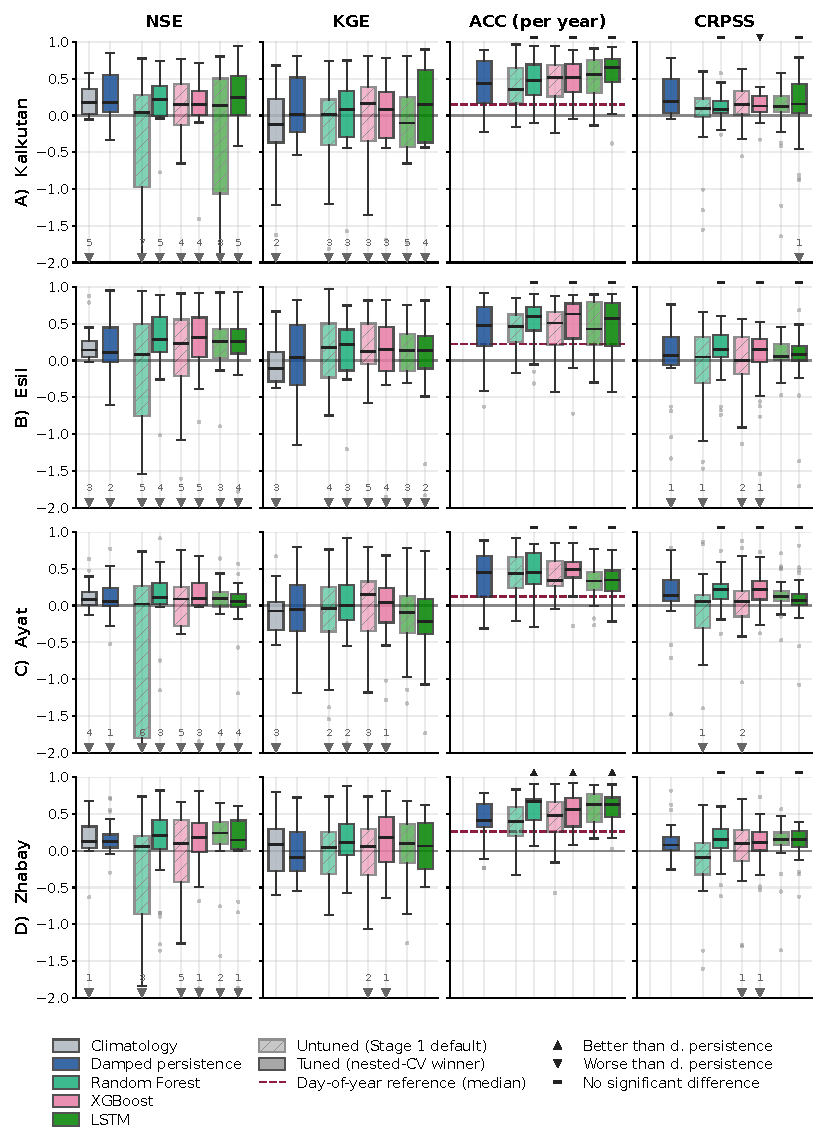
\includegraphics[width=\textwidth,height=0.8\textheight,keepaspectratio]{00_appendix/figB05.pdf}
    \caption{As Figure~\ref{fig:tune_short} (effect of hyperparameter tuning, pooled over lead days 0--30), for the Central Asian nival-dominated steppe catchments (A: Kalkutan; B: Esil; C: Ayat; D: Zhabay).}
    \label{fig:appB_short_steppe}
\end{figure}

\begin{figure}[!htbp]
    \centering
    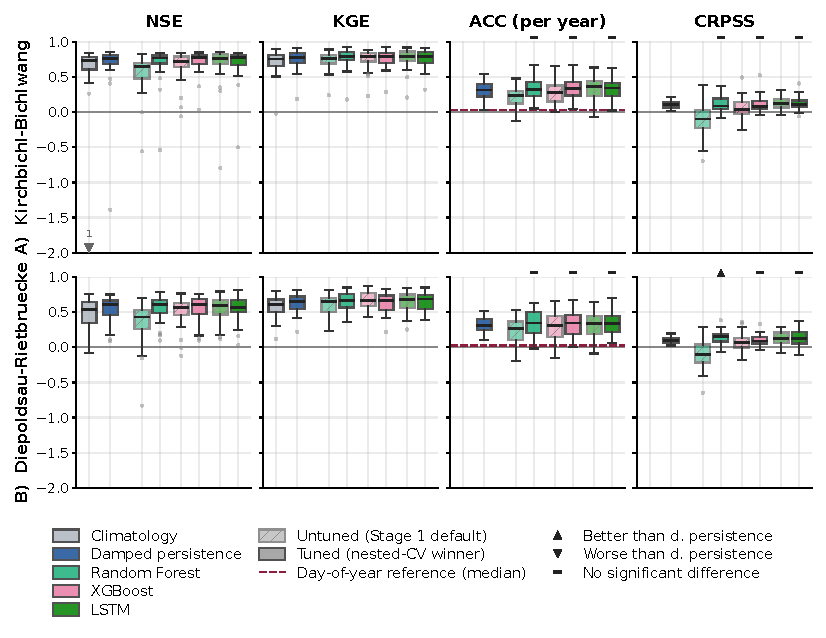
\includegraphics[width=\textwidth]{00_appendix/figB06.pdf}
    \caption{As Figure~\ref{fig:tune_short} (effect of hyperparameter tuning, pooled over lead days 0--30), for the European nival--glacial-dominated mountain catchments (A: Kirchbichl--Bichlwang; B: Diepoldsau--Rietbr\"ucke).}
    \label{fig:appB_short_europe}
\end{figure}

\begin{figure}[!htbp]
    \centering
    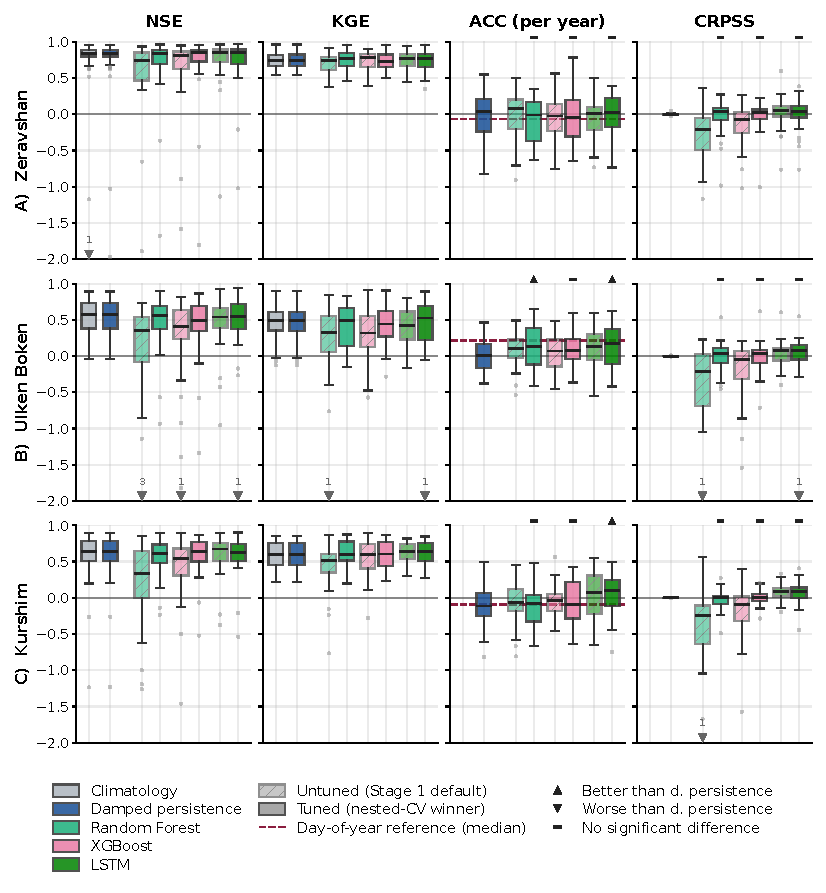
\includegraphics[width=\textwidth]{00_appendix/figB07.pdf}
    \caption{As Figure~\ref{fig:tune_long} (effect of hyperparameter tuning, pooled over lead days 185--214), for the Central Asian nival--glacial-dominated mountain catchments (A: Zeravshan; B: Ulken Boken; C: Kurshim).}
    \label{fig:appB_long_mountain}
\end{figure}

\begin{figure}[!htbp]
    \centering
    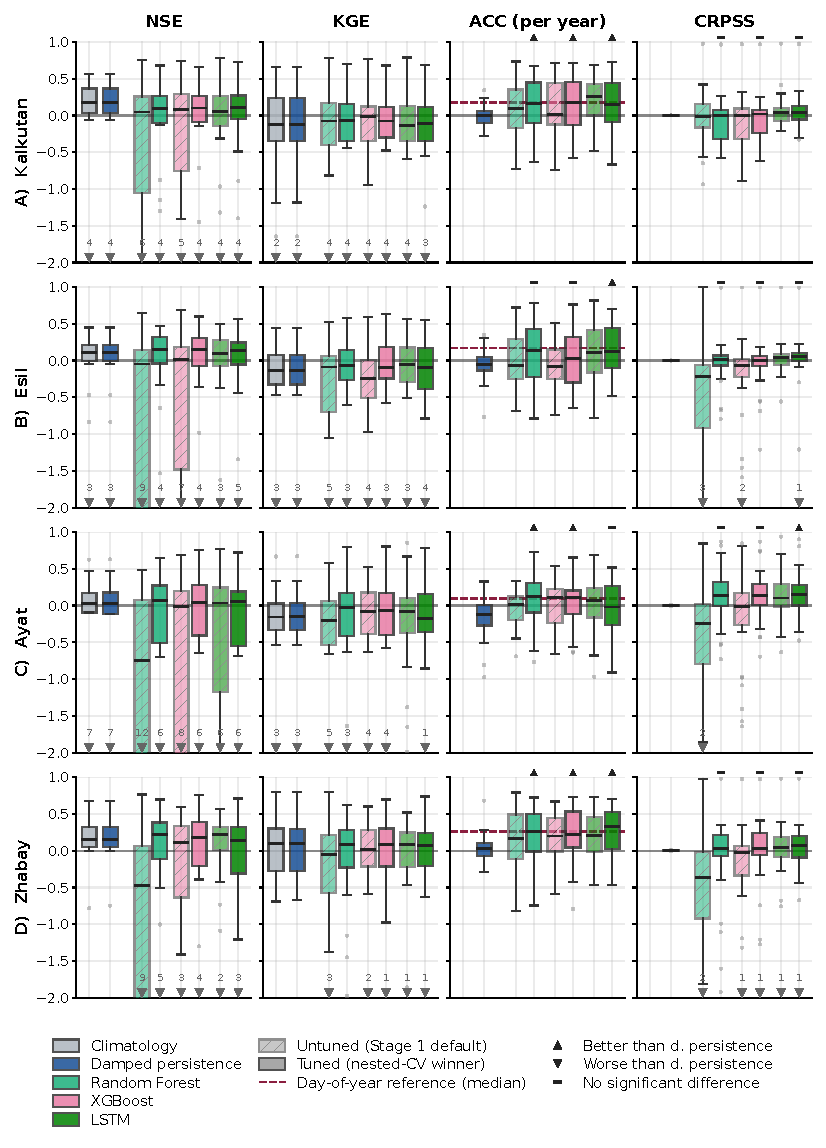
\includegraphics[width=\textwidth,height=0.8\textheight,keepaspectratio]{00_appendix/figB08.pdf}
    \caption{As Figure~\ref{fig:tune_long} (effect of hyperparameter tuning, pooled over lead days 185--214), for the Central Asian nival-dominated steppe catchments (A: Kalkutan; B: Esil; C: Ayat; D: Zhabay).}
    \label{fig:appB_long_steppe}
\end{figure}

\begin{figure}[!htbp]
    \centering
    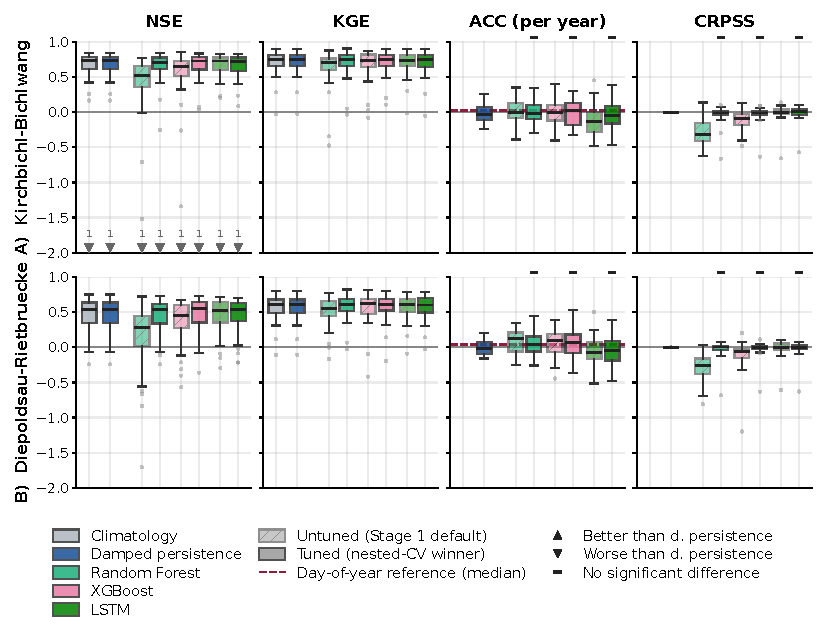
\includegraphics[width=\textwidth]{00_appendix/figB09.pdf}
    \caption{As Figure~\ref{fig:tune_long} (effect of hyperparameter tuning, pooled over lead days 185--214), for the European nival--glacial-dominated mountain catchments (A: Kirchbichl--Bichlwang; B: Diepoldsau--Rietbr\"ucke).}
    \label{fig:appB_long_europe}
\end{figure}

\clearpage

\section{Stage 3 results for all catchments}
\label{app:stage3}
\setcounter{figure}{0}

This appendix extends Section~\ref{sec:results_st3} to all nine study catchments. The main-text figure is repeated once per hydrological regime: the Central Asian nival--glacial-dominated mountain catchments (Zeravshan, Ulken Boken, Kurshim), the Central Asian nival-dominated steppe catchments (Kalkutan, Esil, Ayat, Zhabay), and the European nival--glacial-dominated mountain catchments (Kirchbichl--Bichlwang, Diepoldsau--Rietbr\"ucke). Figures~\ref{fig:appC_sens_mountain}--\ref{fig:appC_sens_europe} show, for each learned model, the per-fold difference between the scores obtained with the original and with the donor-year forcing, over the full forecast horizon (lead days 0--214). Metrics, symbols and sign conventions are as described for Figure~\ref{fig:sensitivity}.

\begin{figure}[!htbp]
    \centering
    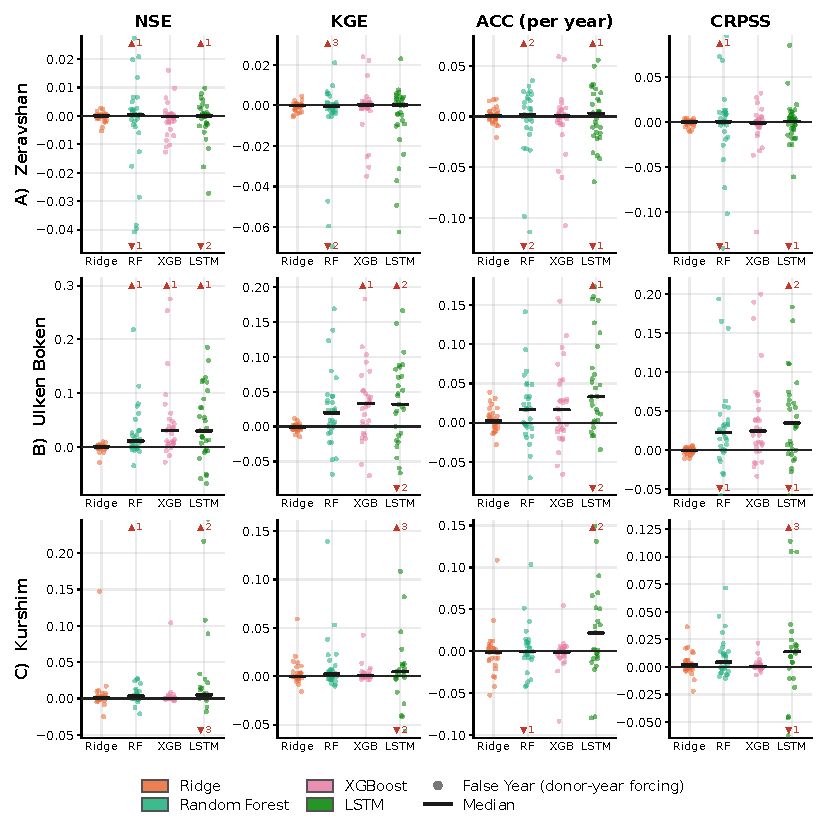
\includegraphics[width=\textwidth]{00_appendix/figC01.pdf}
    \caption{As Figure~\ref{fig:sensitivity} (sensitivity to the meteorological forcing, lead days 0--214), for the Central Asian nival--glacial-dominated mountain catchments (A: Zeravshan; B: Ulken Boken; C: Kurshim).}
    \label{fig:appC_sens_mountain}
\end{figure}

\begin{figure}[!htbp]
    \centering
    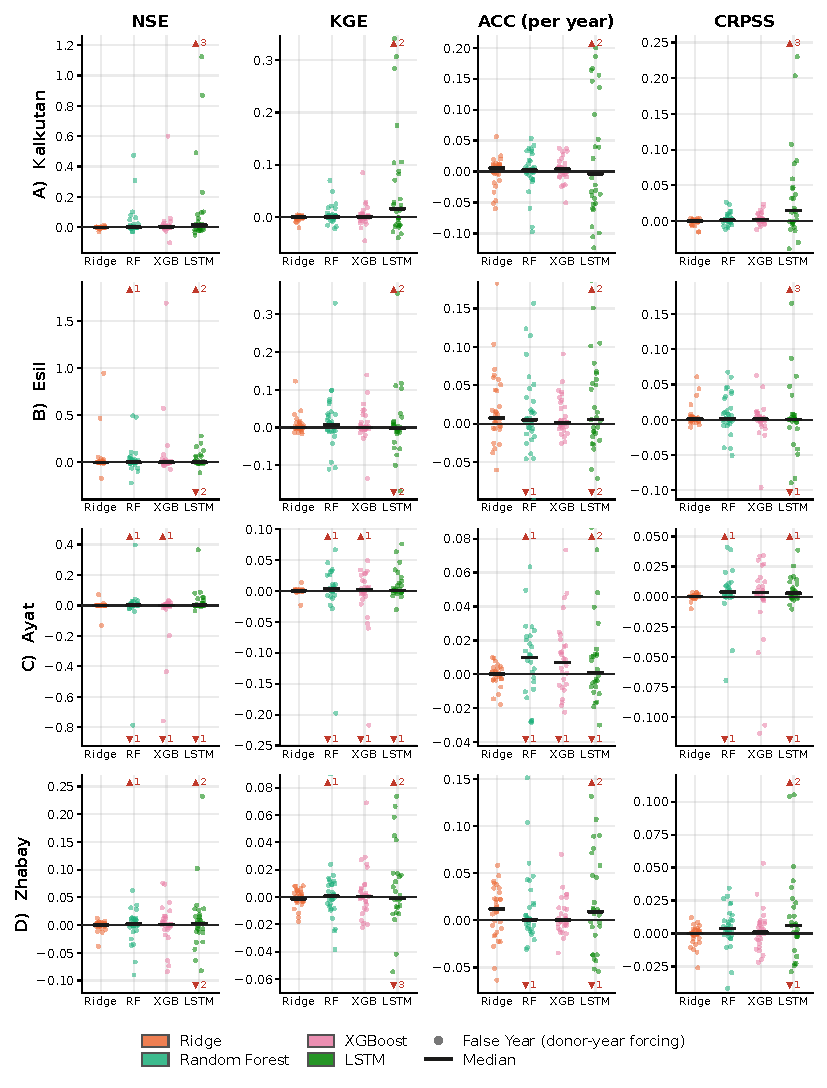
\includegraphics[width=\textwidth,height=0.8\textheight,keepaspectratio]{00_appendix/figC02.pdf}
    \caption{As Figure~\ref{fig:sensitivity} (sensitivity to the meteorological forcing, lead days 0--214), for the Central Asian nival-dominated steppe catchments (A: Kalkutan; B: Esil; C: Ayat; D: Zhabay).}
    \label{fig:appC_sens_steppe}
\end{figure}

\begin{figure}[!htbp]
    \centering
    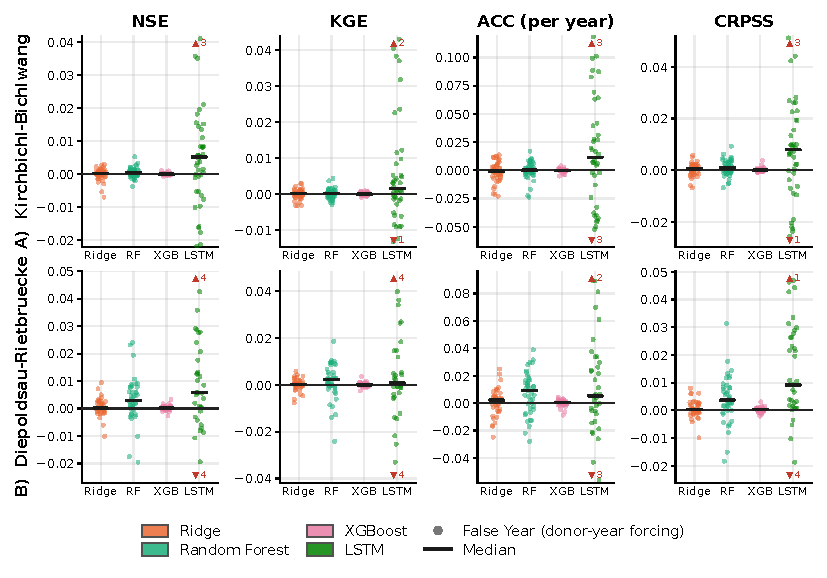
\includegraphics[width=\textwidth]{00_appendix/figC03.pdf}
    \caption{As Figure~\ref{fig:sensitivity} (sensitivity to the meteorological forcing, lead days 0--214), for the European nival--glacial-dominated mountain catchments (A: Kirchbichl--Bichlwang; B: Diepoldsau--Rietbr\"ucke).}
    \label{fig:appC_sens_europe}
\end{figure}

\clearpage



%% --- References ---
%% If you have bib database file and want bibtex to generate the
%% bibitems, please use
%%
%%  \bibliographystyle{elsarticle-harv} 
%%  \bibliography{<your bibdatabase>}

%% else use the following coding to input the bibitems directly in the
%% TeX file.

%% Refer following link for more details about bibliography and citations.
%% https://en.wikibooks.org/wiki/LaTeX/Bibliography_Management

\bibliographystyle{elsarticle-harv}
\bibliography{references}

\end{document}

\endinput
%%
%% End of file `elsarticle-template-harv.tex'.


